\documentclass[a4paper,12pt]{report}

%encoding
%--------------------------------------
\usepackage[utf8]{inputenc}
\usepackage[T1]{fontenc}
\usepackage{graphicx}
\usepackage{indentfirst}
\usepackage[export]{adjustbox}
\usepackage{float}
%--------------------------------------
 
%Portuguese-specific commands
%--------------------------------------
\usepackage[portuguese]{babel}
%--------------------------------------
\setcounter{secnumdepth}{4}
\setcounter{tocdepth}{4}

% Define o autor e tıtulo
\author{
  Octávio Maia\\
  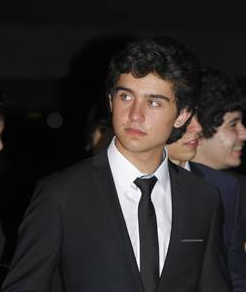
\includegraphics[width=0.27\textwidth]{media/capa/octavio.PNG}
  \\\texttt{a71369}
  \and
  João Silva\\
  
\includegraphics[width=0.25\textwidth]{media/capa/joao.png}
  \\\texttt{a72023}
  \and
  Rui Freitas\\
  
\includegraphics[width=0.274\textwidth]{media/capa/rui.png}
  \\\texttt{a72399}
  \and
  Pedro Pinto\\
  
\includegraphics[width=0.29\textwidth]{media/capa/pinto.jpg}
  \\\texttt{a71929}
  \and
  Nuno Oliveira\\
  
\includegraphics[width=0.25\textwidth]{media/capa/nuno.jpg}
  \\\texttt{a72028}
}

\title{
	%
\includegraphics[width=0.5\textwidth]{media/capa/logo_eeng.png}
	%\\
	\textbf{Desenvolvimento de Sistemas de Software\\MIEINF\\}
	\textbf{2015/2016}
}


\begin{document}

\maketitle
\tableofcontents
 

\newpage

\chapter{Parte 1}

\section{Introdução}

Este trabalho prático tem como base a criação de um sistema de suporte à realização de eleições.
\\\indent Como indicado no enunciado o sistema possui dois modos distintos de funcionamento.
\begin{itemize}
\item Permite a criação de um ato eleitoral, permitindo definir o tipo de eleição, candidatos, listas, partidos, data limite, entre outros.
\item Por outro, permite também a gerência do ato eleitoral, ou seja, permite o registo de votos, atribuição de mandatos, cálculo do vencedor, criação de segunda volta, entre outros.
\end{itemize}
\indent Como referido no enunciado, os dois modos de funcionamento foram disponibilizados numa única aplicação, havendo distinção entre os votantes e os administradores do sistema. 
\\\indent A aplicação em causa tem como base as normas disponibilizadas no site da Comissão Nacional de Eleições\footnote{http://www.cne.pt/content/legislacao-eleitoral}, para os atos eleitorais realizados em Portugal e suporta dois tipos de eleição:
\begin{enumerate}
\item Assembleia da República
\item Presidência da República
\end{enumerate}
Nesta fase do projeto iremos entregar a fase inicial do projeto, contendo os Modelos de Domínio/Use Case, bem como os Diagramas de Sequencia Software/Máquinas de Estado e uma proposta da futura interface \emph{Mockup}.

\newpage

\section{Modelo de Domínio}
O modelos de domínio que propomos, são os apresentados de seguida que tentam abordar todos os aspetos importantes para o suporte das funcionalidades que é suposto a aplicação dar suporte, e ao mesmo tempo captar todos os aspetos legais importantes para seguir esses requisitos, abstraindo de aspetos não essenciais para a aplicação, tais como a gestão de tarefas administrativas e burocráticas.
\subsection{Assembleia da República}

O modelo de domínio da Assembleia da República é representado por uma eleição, que é efectuada numa determinada data, e tem um caderno de recenceamento, onde contém as informações de todos os cidadãos permitidos a votar. Cada eleição cria um mapa de eleição quando iniciada, e preenche uma assembleia. As assembleias são constituídas por deputados, cada um deles correspondentes a um mandato, eleito por um círculo eleitoral. Cada círculo eleitoral pode ou não ter listas candidatas a Assembleia. Cada lista pode ser singular, se for constituída por apenas um partido, ou pode tratar-se de uma coligação, caso o número de partidos seja maior que 1. Tanto os partidos como as coligações são distinguidos pela sua nominação, símbolo e sigla. Os partidos são liderados por um lider, que por sua vez pode também ser um eleitor. Existe um candidato suplente, para prevenir situações irregulares que possam aconteçer com o candidato principal. Para identificação dos candidatos, decidimos atribuir-lhes idade, profissão, residência, naturalidade, filiação, e o número de cartão de cidadão. 
\\\indent A ordem de apresentação no boletim de voto de cada círculo eleitoral é gerada através de um sorteio. O boletim de voto é o espaço onde os eleitores podem deixar o seu voto. Voto este que pode ser válido, quando apenas é selecionado um partido no boletim de voto; branco, quando não é selecionado nenhum partido; e nulo, quando o voto do eleitor não é válido. No nosso projeto, cada eleitor é identificado por um número identificador, um PIN e pelo seu nome.

\begin{figure}[h]
\begin{center}
	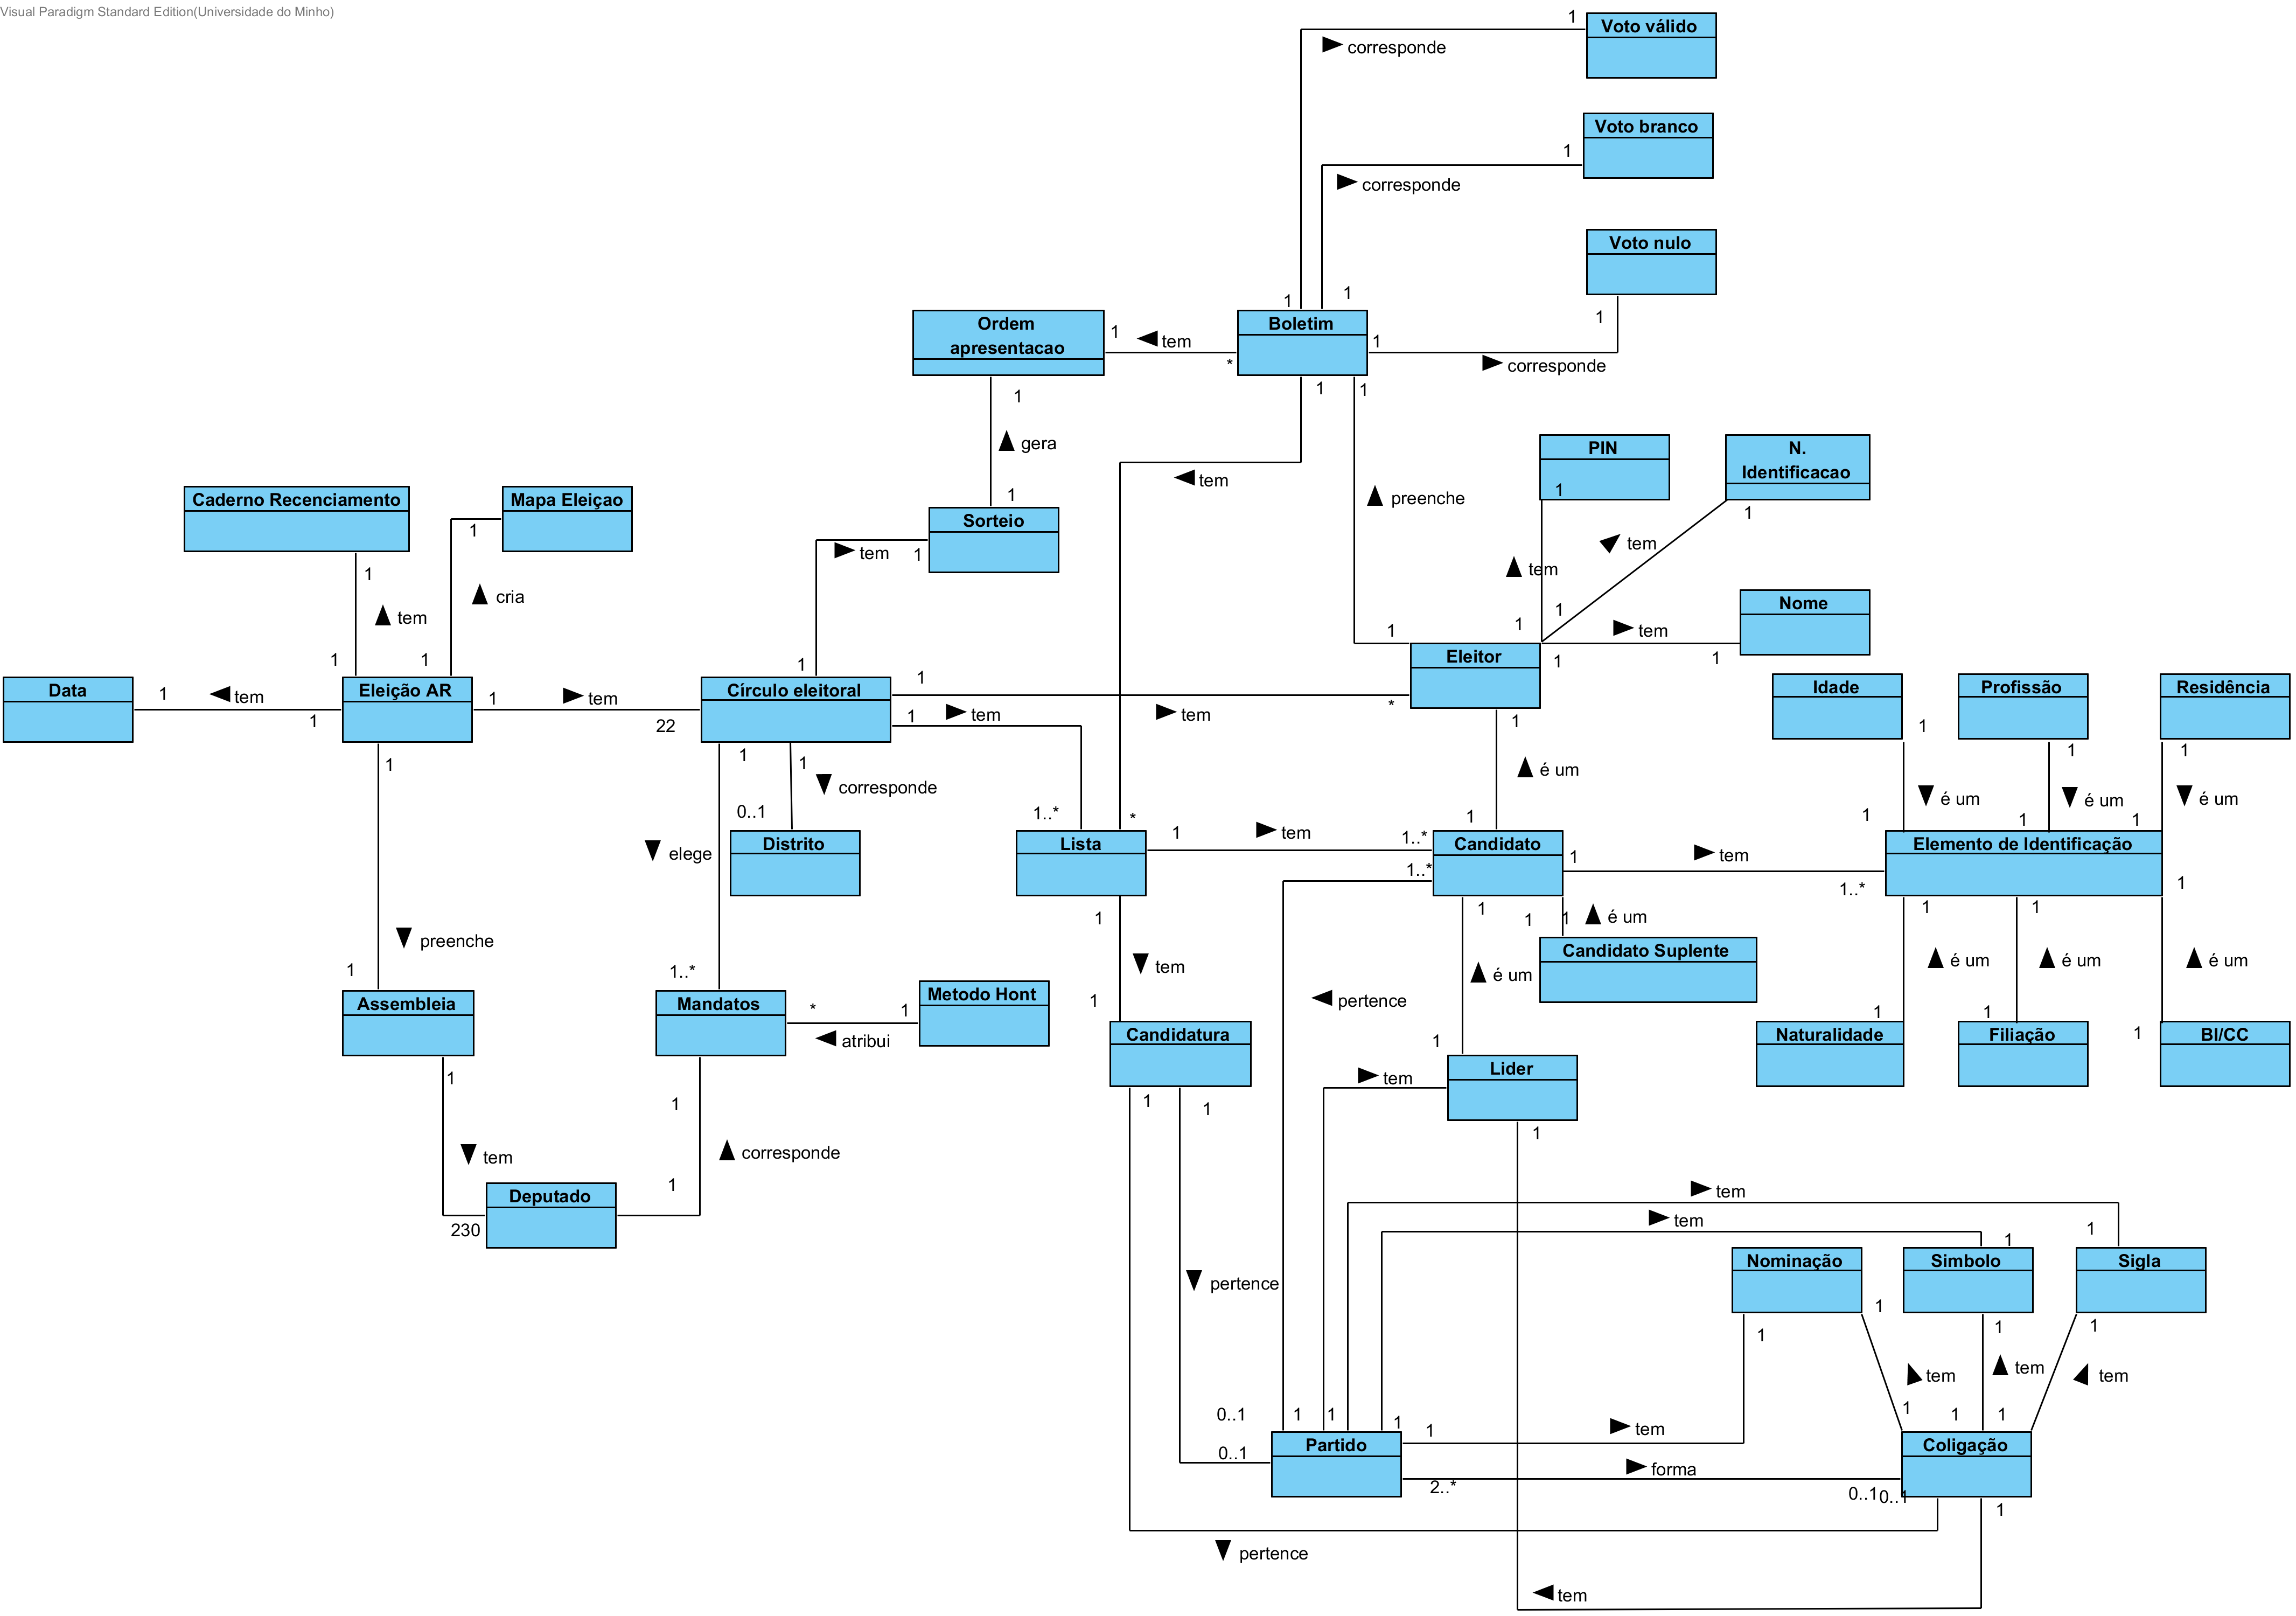
\includegraphics[width=0.7\textwidth]{media/modelodominio/ar.png}
	 \caption{Modelo de Domínio da Assembleia da República.}
\end{center}
\end{figure}

\newpage
\subsection{Presidência da República}
O modelo de domínio para às eleições da Presidência da República o grupo decidiu que toda a informação relativa aos eleitores deveria ser mantida igual as eleições da \textbf{Assembleia da República}, mesmo que não seja totalmente necessária para este tipo de eleição, como a informação relativa ao círculo pertencente a que pertence cada eleitor isso também facilitaria todo o processo de gestão dos cadernos de recenseamento que passa a ser igual. Por outro lado ao mantendo a informação dos círculos podemos oferecer na parte de consulta de resultados eleitorais informação com mais detalhe para cada círculo eleitoral.
\\\indent Em questões mais relacionadas com a tipologia da eleição, esta é mais simples que a eleição da \textbf{Assembleia da República}, pois as listas que são apresentadas, são comuns a todo o país, eliminado a necessidade de diferenciar as listas para cada círculo e gestão dos boletins de voto. Também esta eleição na sua essência a lista é apenas constituída pelo candidato que concorre à presidência não sendo necessário no nosso ponto de vista a aplicação guardar toda a restante informação, como quem apoiou a candidatura.
\\\indent Outra diferença relativa as eleições da \textbf{Assembleia da República} é pelo facto de caso não seja obtida maioria absoluta na primeira volta por parte de um candidato ser necessário recorrer a uma nova eleição de segunda volta entre os dois candidatos mais votados na primeira volta, sendo certo que nesta segunda volta a decisão da eleição é tomada. 
\begin{figure}[h]
\begin{center}
	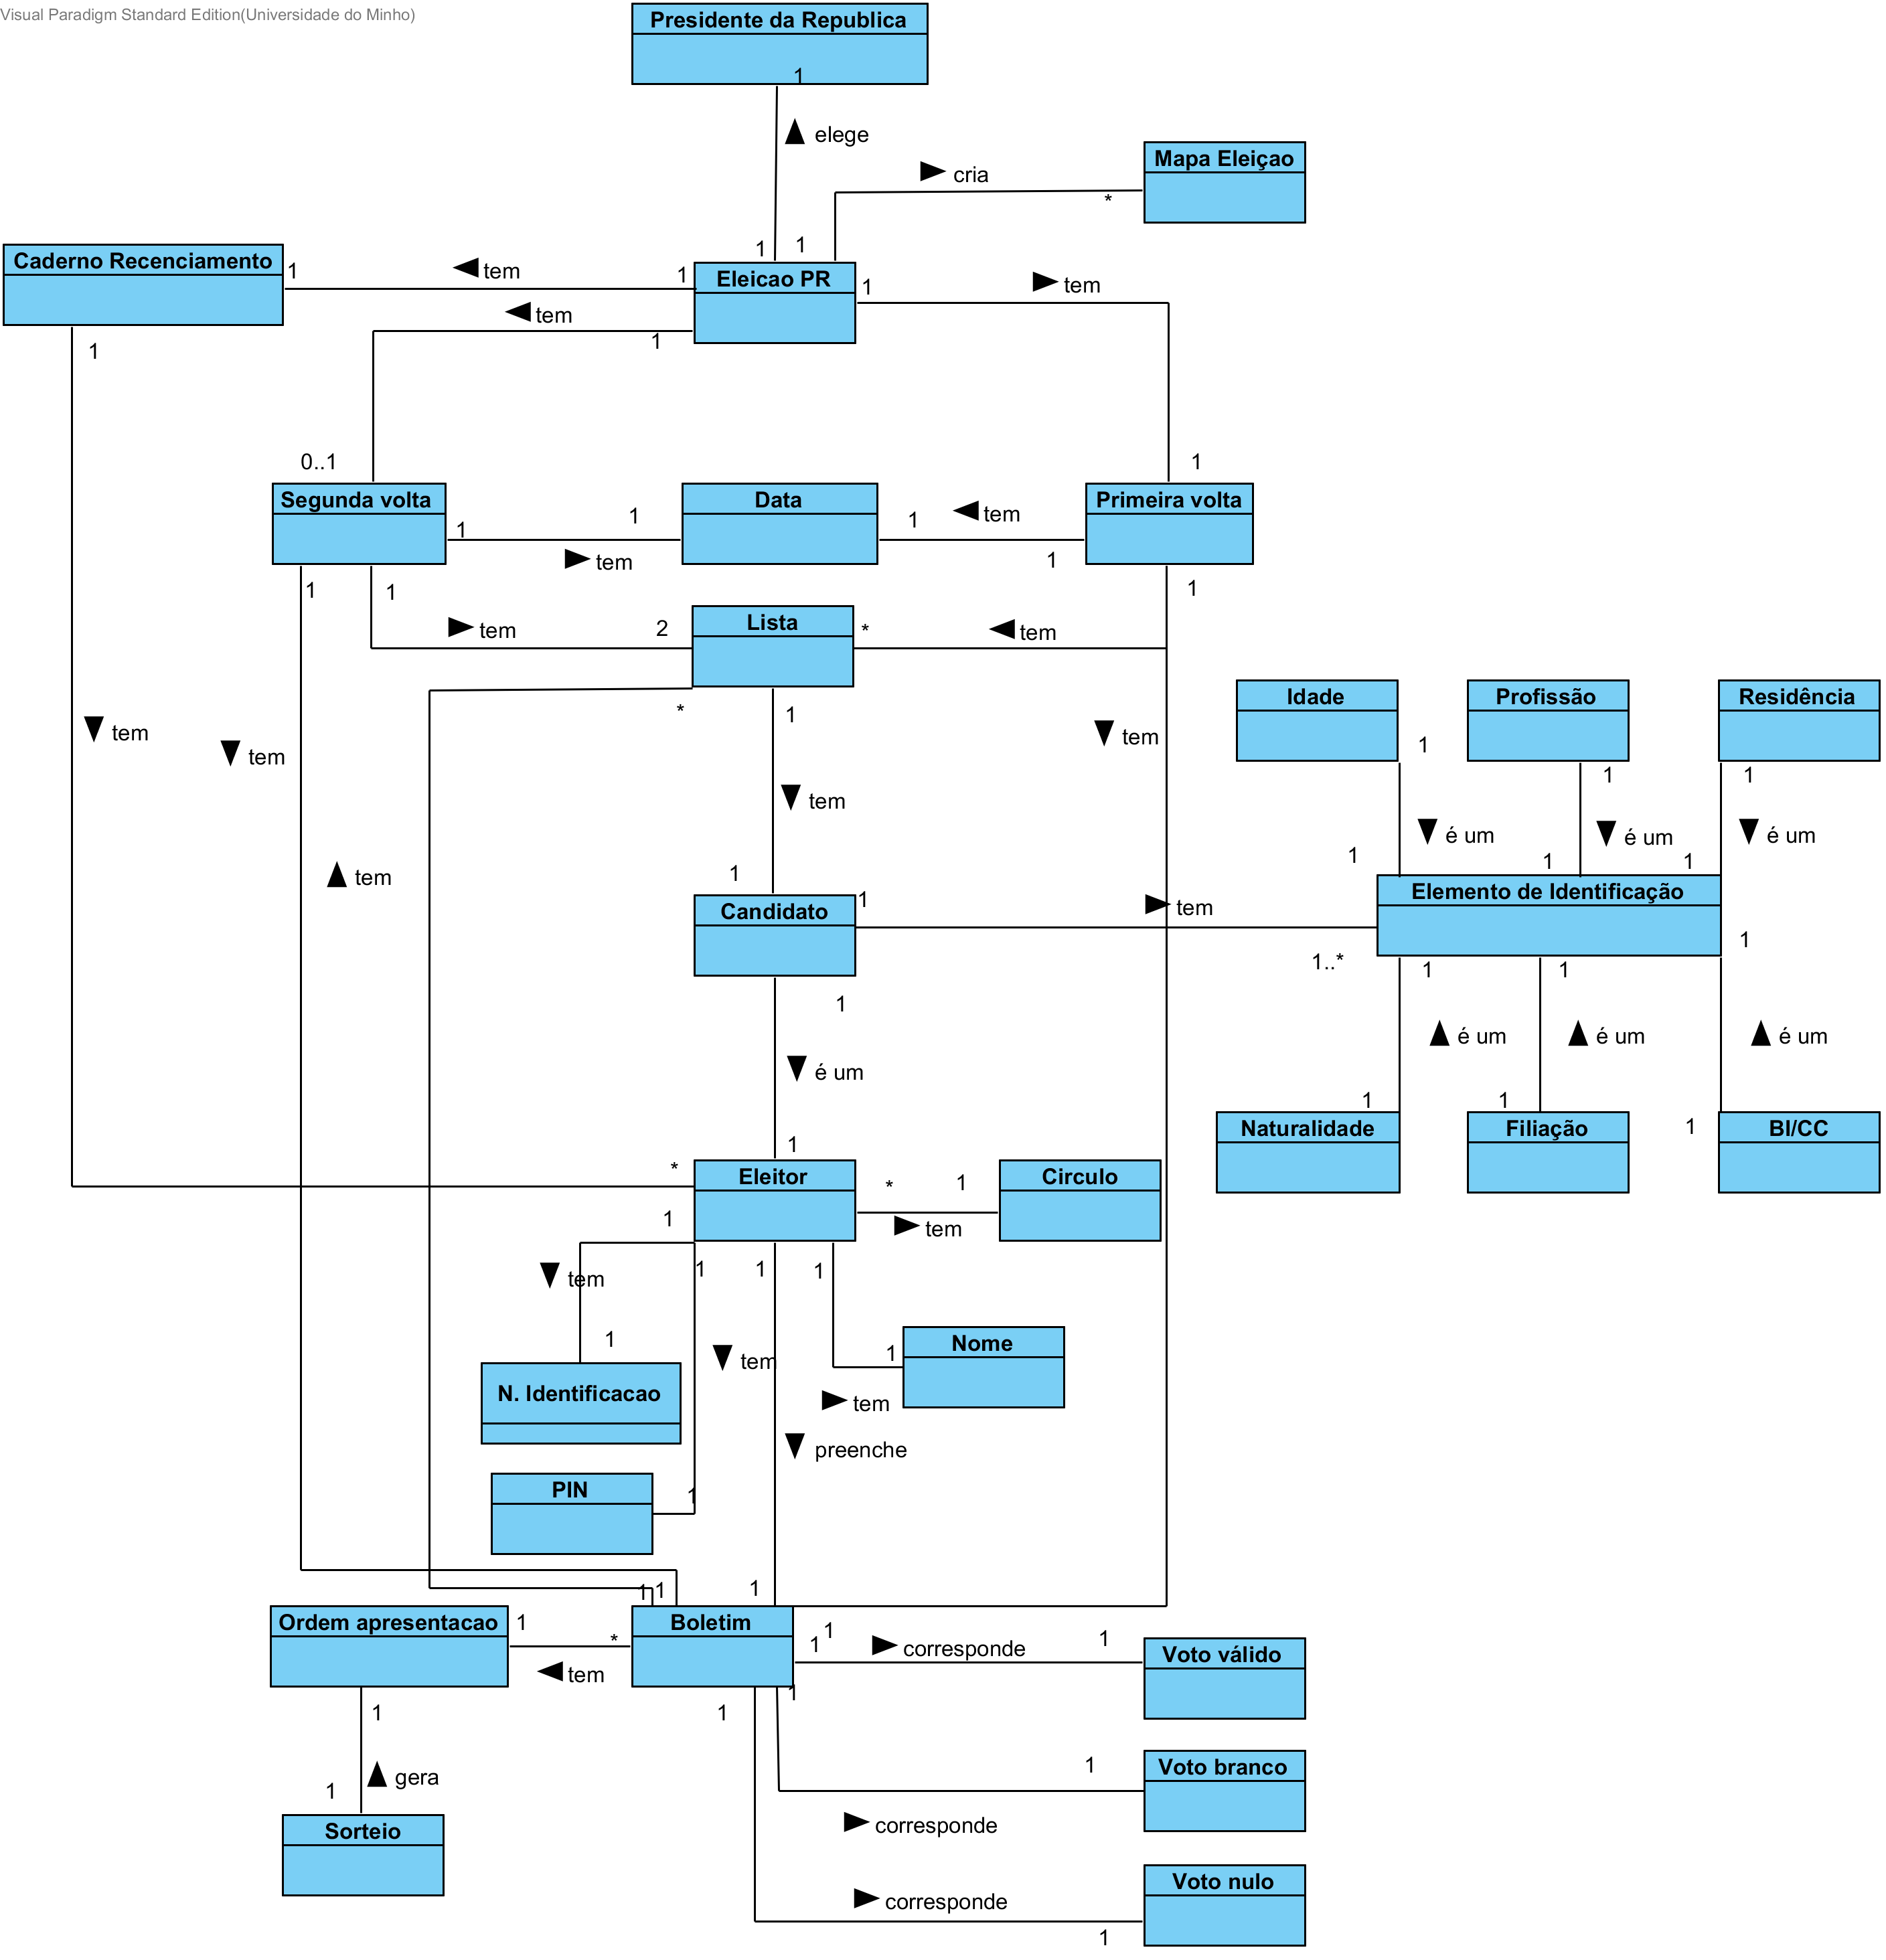
\includegraphics[width=0.55\textwidth]{media/modelodominio/pr.png}
	 \caption{Modelo de Domínio da Presidência da República.}
\end{center}
\end{figure}

\clearpage
\section{Modelos de Use Case e Diagramas de Sequência Software}
Nesta secção definimos o modo de funcionamento da nossa aplicação. Aqui já começamos a pensar um pouco nas classes ou subsistemas que vamos utilizar.
Entre os vários use cases criados, destacamos os seguintes:

\subsection{Cria Eleição}
Neste Use Case, o primeiro passo é pedir ao Administrador a data de início da eleição, a data de fim, os partidos participantes e as listas.
\\\indent Após a obtenção de toda esta informação o subsistema de eleições cria a Eleição.
\\\indent Mesmo após a eleição ter sido criada, é possível adicionar novas listas. Isto é feito pedindo ao sistema de eleições a adição de uma nova lista, que por sua vez pede ao subsistema de círculos a adição da lista. Após o subsistema de círculos adicionar a lista este reporta ao subsistema de eleições a adição com sucesso, que por sua vez reporta à interface.

\begin{figure}[h]
\begin{center}
	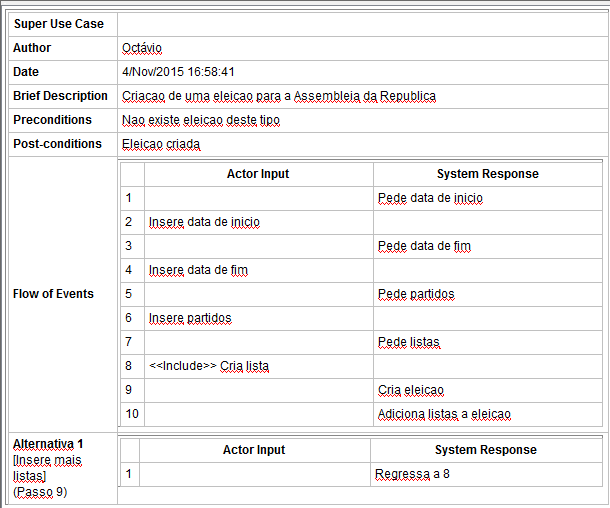
\includegraphics[width=0.5\textwidth]{media/usecase_dss/uc_criaEleicao.PNG}
	 \caption{Diagrama de Use Case do Cria Eleição.}
\end{center}
\end{figure}

\begin{figure}[h]
\begin{center}
	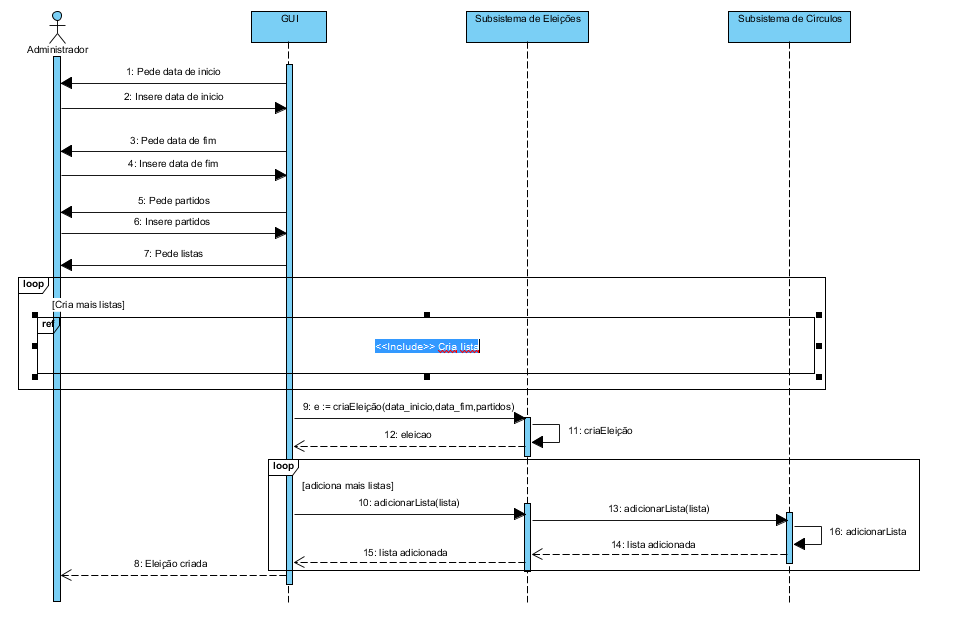
\includegraphics[width=0.5\textwidth]{media/usecase_dss/CriaEleicao.png}
	 \caption{Diagrama de Sequência do Cria Eleição.}
\end{center}
\end{figure}

\newpage
\subsection{Vota (Assembleia da República)}
Neste use case, o primeiro passo é pedir ao subsistema de eleição o boletim de voto do círculo ao qual o eleitor pertence. Para obter essa informação, é necessário ir ao subsistema do eleitor ver o seu círculo e, de seguida, para esse círculo, obter o seu boletim de voto.

Após a obtenção do boletim, este é mostrado ao eleitor, que tem três opções: ou escolhe apenas uma lista e atribui o seu voto, ou não escolhe nenhuma lista e atribui um voto em branco, ou escolhe múltiplas listas, e o voto é nulo. De seguida, o voto é registado na eleição e círculo em questão.

\begin{figure}[h]
\begin{center}
	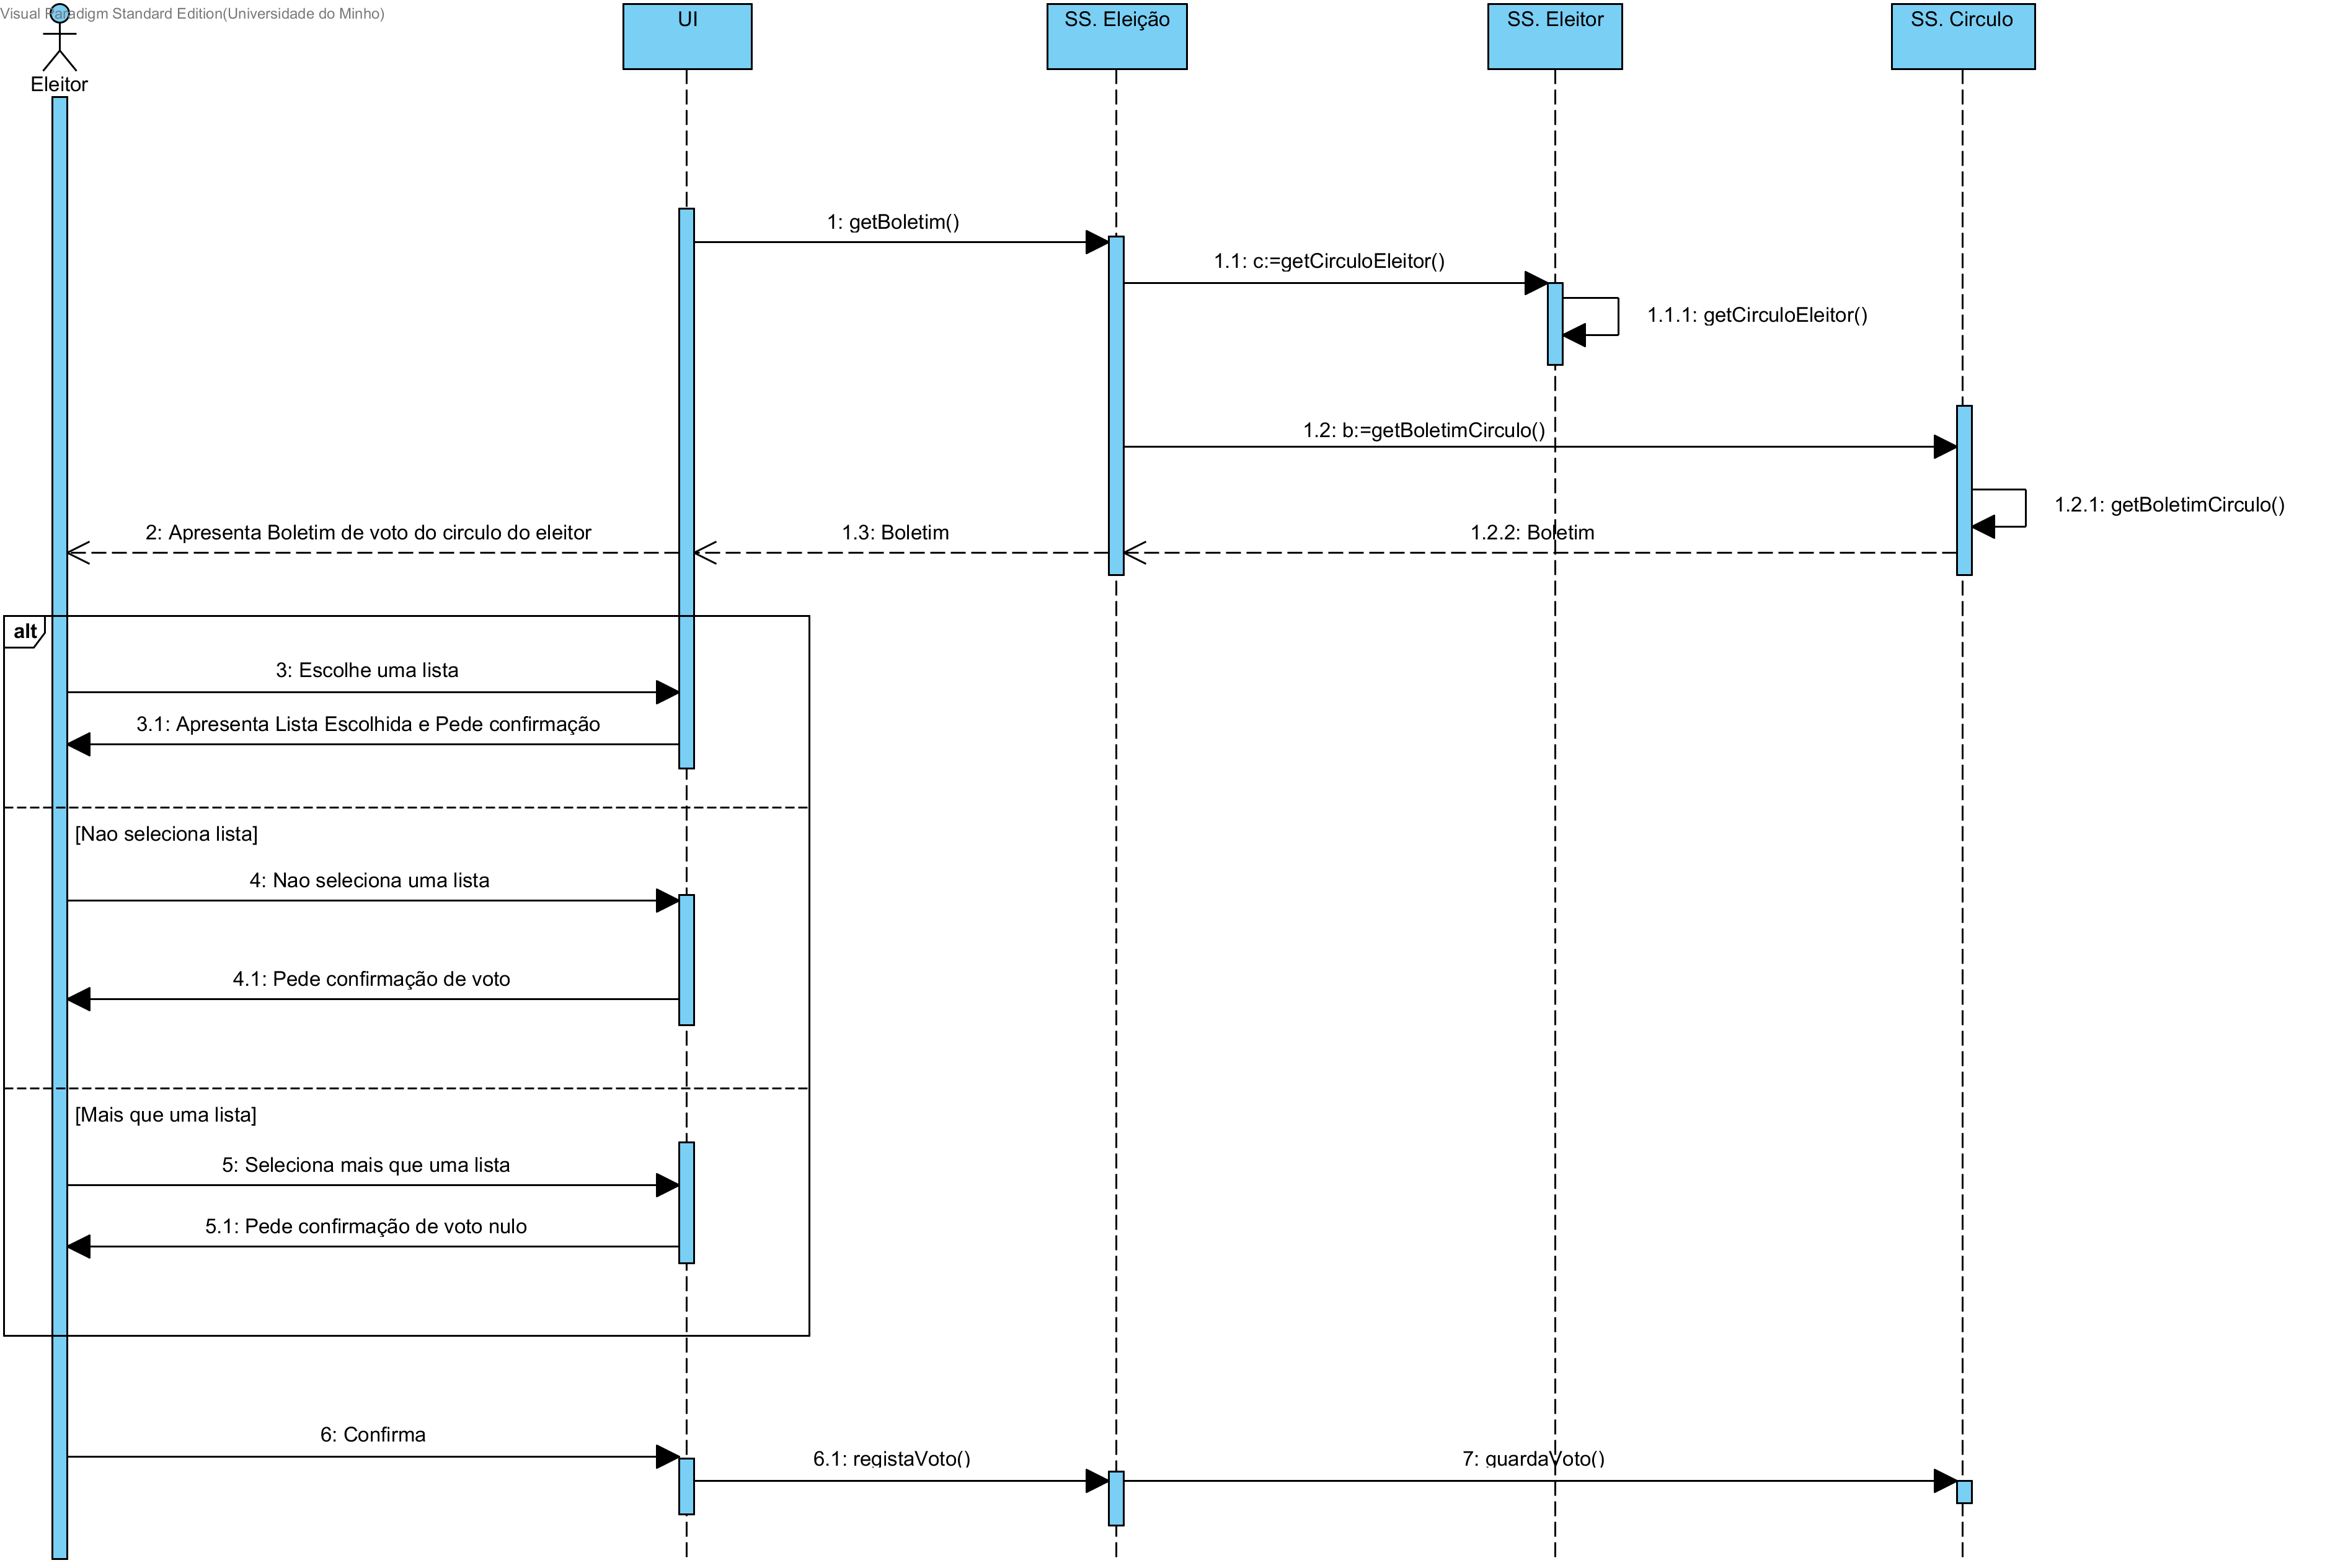
\includegraphics[width=0.5\textwidth]{media/usecase_dss/ar_vota.png}
	 \caption{Diagrama de Sequência do Vota da Assembleia da República.}
\end{center}
\end{figure}

\begin{figure}[h]
\begin{center}
	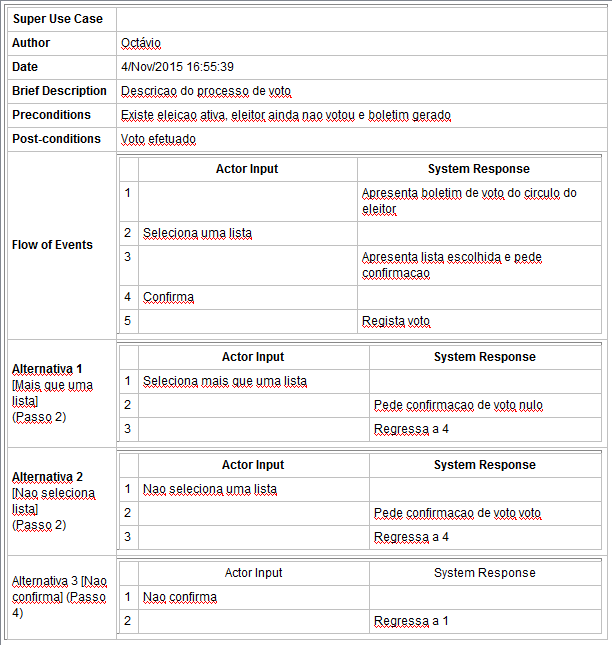
\includegraphics[width=0.5\textwidth]{media/usecase_dss/uc_vota.PNG}
	 \caption{Diagrama de Use Case do Vota da Assembleia da República.}
\end{center}
\end{figure}

\newpage
\section{Proposta de Interface (Mockup) e Máquinas de Estado}
Para este projeto, realizamos uma proposta de interface, utilizando a ferramenta \emph{Evolus Pencil} que iremos apresentar de seguida.

\subsection{Janela de login}

\begin{figure}[h]
\begin{center}
	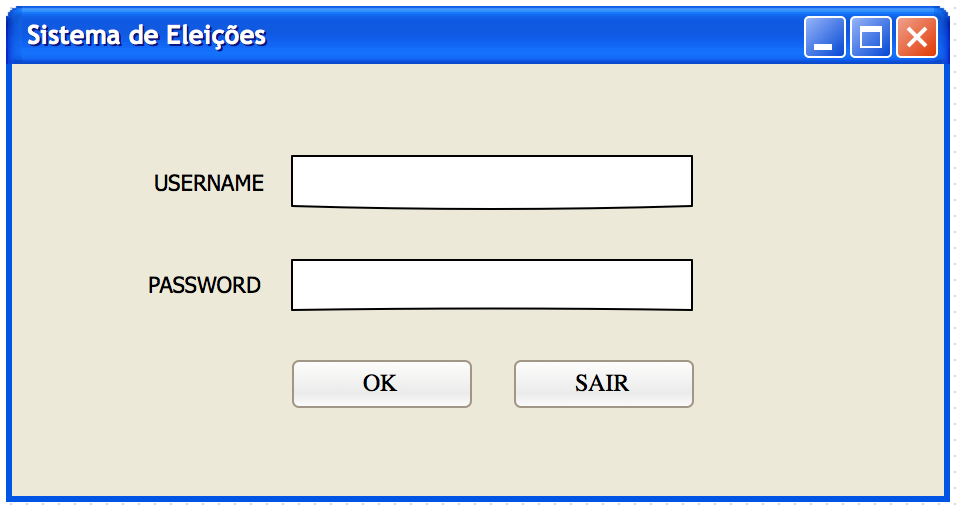
\includegraphics[width=0.5\textwidth]{media/mockup/login.png}
	 \caption{Janela de login.}
\end{center}
\end{figure}

\begin{figure}[h]
\begin{center}
	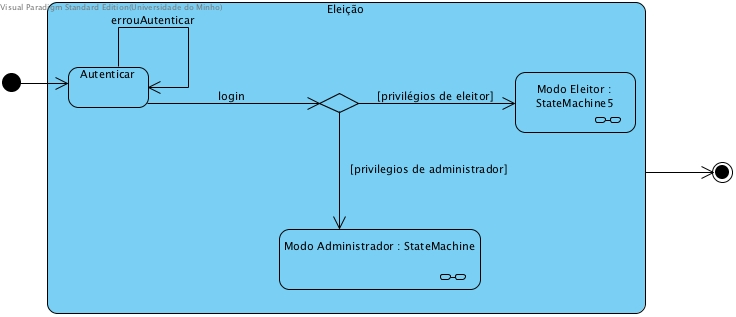
\includegraphics[width=0.5\textwidth]{media/MaqEst/m_interface.jpg}
	 \caption{Maquina de Estado janela de login.}
\end{center}
\end{figure}

Esta é a janela proposta de login, janela esta que distingue automaticamente os Administradores do sistema dos restantes votantes, tendo cada um acesso a partes diferentes do programa.

\newpage
\subsection{Gestão de eleição (Administrador)}

Após o login do Administrador, este é apresentado com uma janela em que é apresentada a eleição ativa (caso exista), que permite o término da mesma.
\\\indent Numa segunda parte da mesma janela são apresentadas todas as eleições criadas e ativas bem como as eleições já terminadas.
\\\indent Caso esteja no separador de eleições criadas é possível iniciar a eleição, criar uma nova eleição e gerir a mesma.
\\\indent Uma outra parte da janela é relativa às eleições já realizadas, que permite a visualização dos resultados de uma aquando selecionada.
\\\indent Em qualquer momento, nesta janela, o Administrador pode inserir uma nova versão do Caderno de Recenseamento. 

\begin{figure}[h]
\begin{center}
	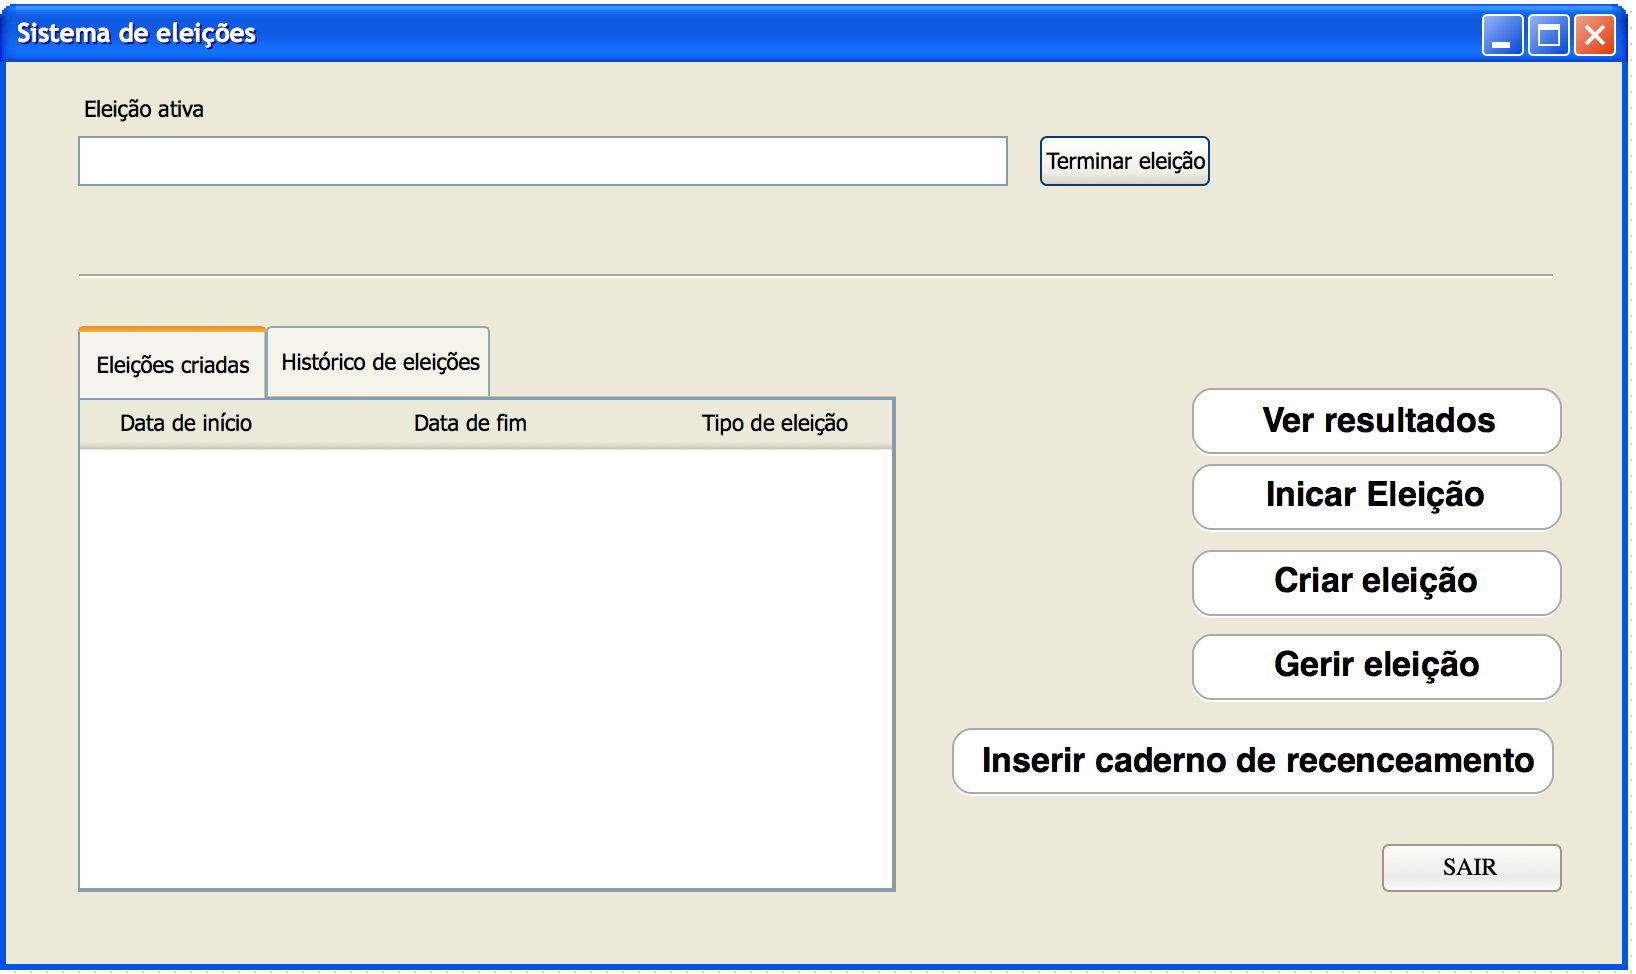
\includegraphics[width=0.5\textwidth]{media/mockup/MainAdmin.png}
	 \caption{Janela principal do Administrador.}
\end{center}
\end{figure}
\begin{figure}[h]
\begin{center}
	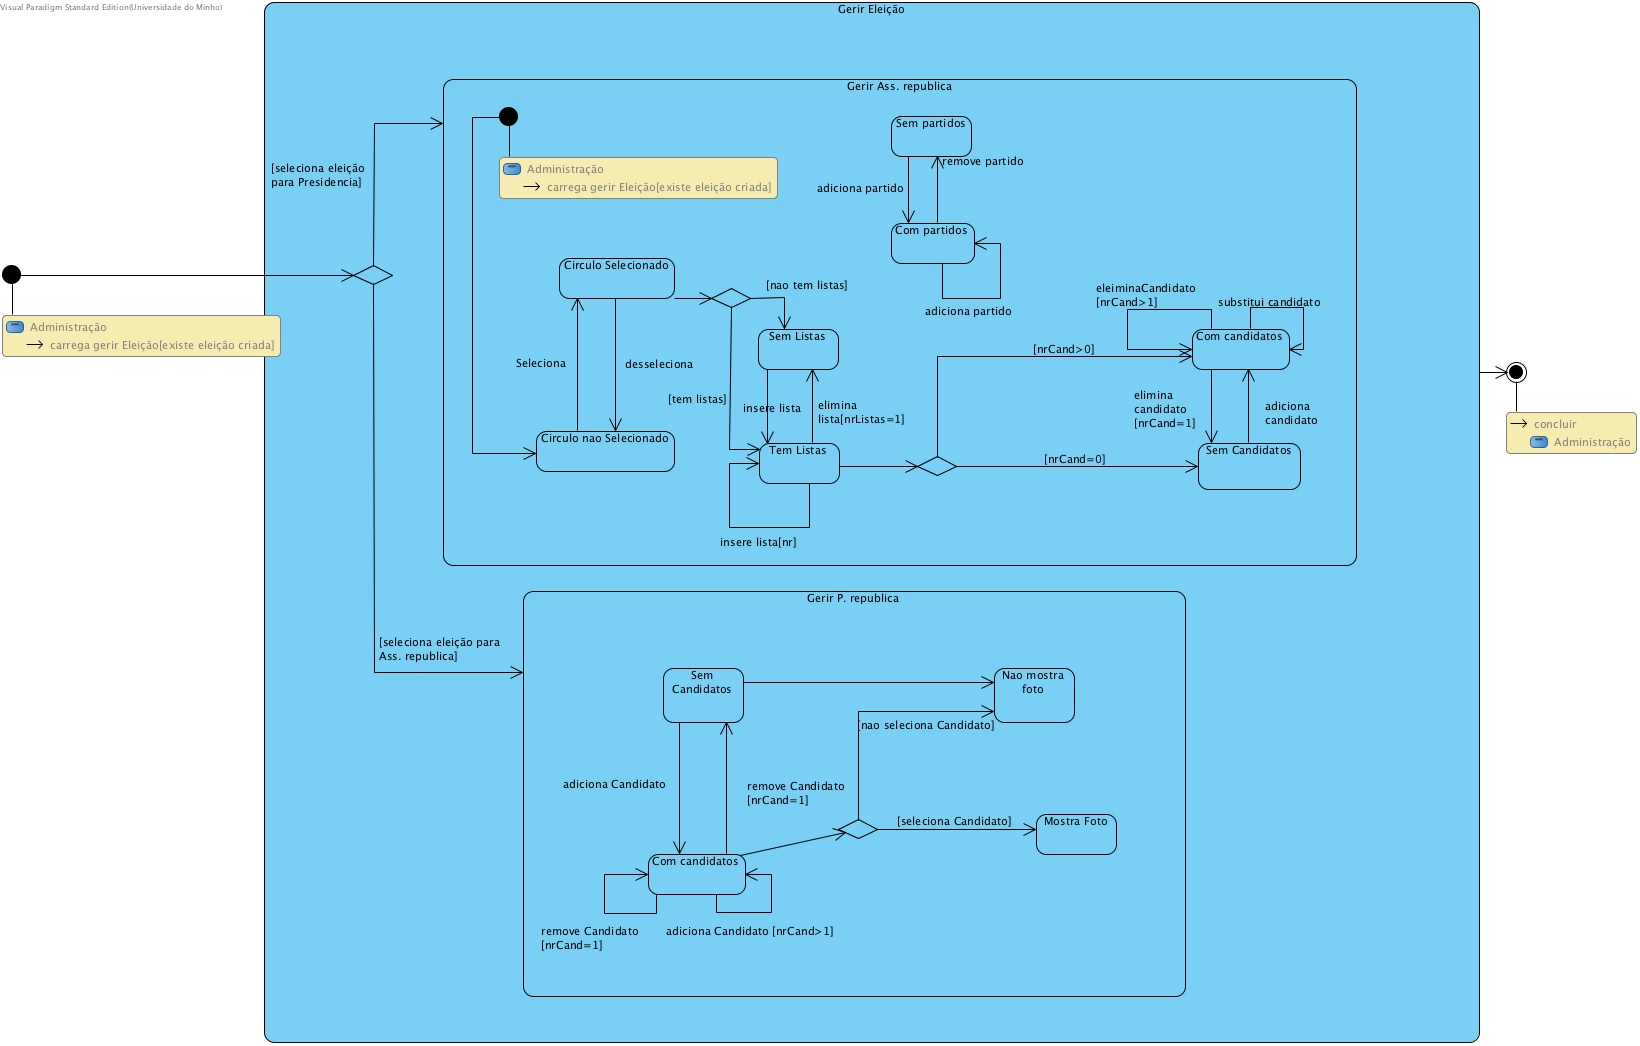
\includegraphics[width=0.5\textwidth]{media/MaqEst/m_GerirEleicao.jpg}
	 \caption{Maquina de Estado janela principal do Administrador.}
\end{center}
\end{figure}

\newpage
\subsubsection{Criar Eleição}
A janela de criação de eleição é a mesma para os dois tipos de eleição, o administrador uma vez nesta janela tem a possibilidade de escolher o tipo de eleição a criar (Assembleia da República ou Presidência da República), o Administrador terá também necessariamente inserir a data da eleição.
\begin{figure}[h]
\begin{center}
	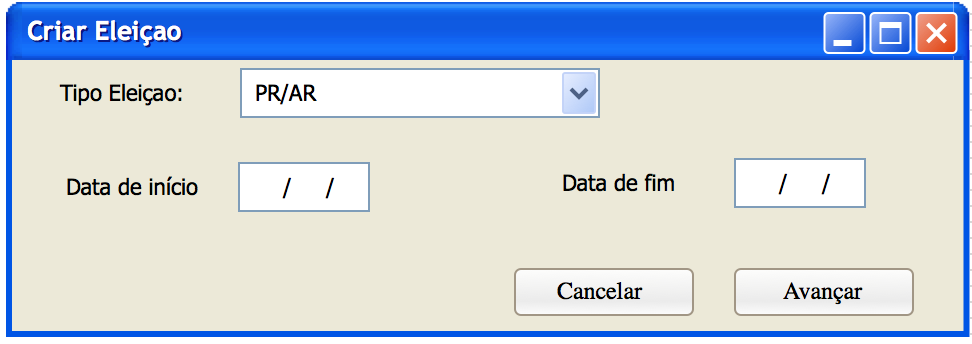
\includegraphics[width=0.5\textwidth]{media/mockup/CriarEleicao.png}
	 \caption{Janela de Criação de eleições.}
\end{center}
\end{figure}
\begin{figure}[h]
\begin{center}
	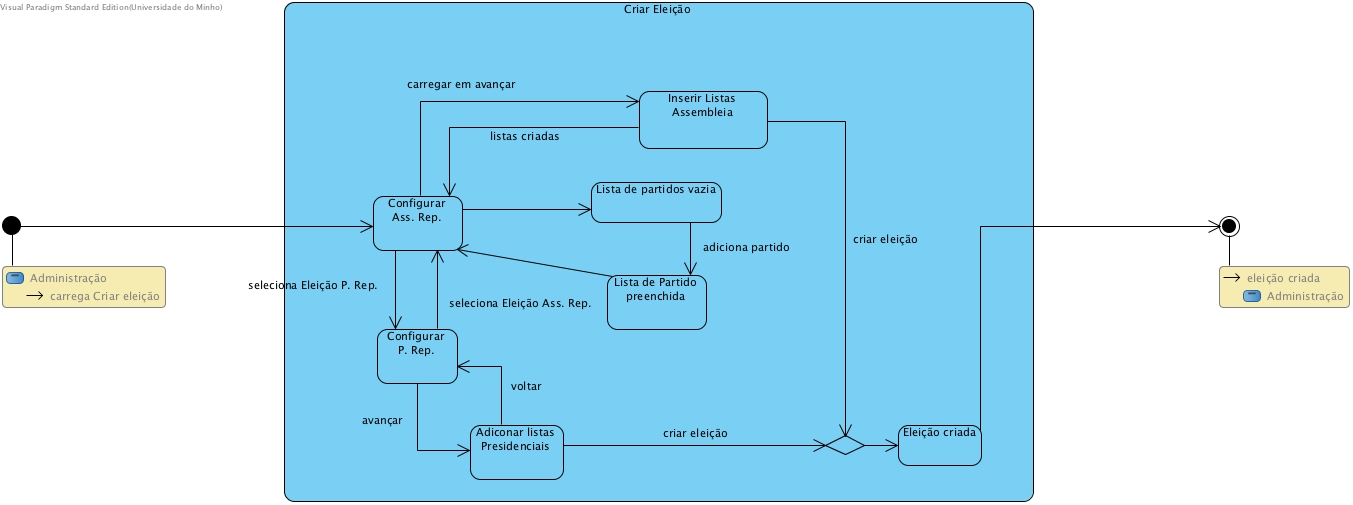
\includegraphics[width=0.5\textwidth]{media/MaqEst/m_CriarEleicao.jpg}
	 \caption{Maquina de estado da Janela de Criação de eleições.}
\end{center}
\end{figure}

\subsubsection{Gerir Eleições da Assembleia da República}
A quando a seleção da gestão de uma eleição por parte do administrador este é direcionado para uma janela igual à apresentada onde o mesmo efetua a todo o processo de gestão das eleições do tipo \emph{Assembleia da República}.
\\\indent Num primeiro passo o Administrador terá de selecionar o circulo que quer gerir, imediatamente é apresentado o numero de mandatos que esse circulo tem direito e também uma lista com a sigla, nome e identificação dos partidos políticos de todas as listas existentes no circulo. Caso o Administrador tenha o desejo de adicionar uma nova lista este deverá inserir o respetivo nome, e sigla bem como selecionar todos os partidos pertencentes a essa lista, caso algum partido que se pretenda adicionar a uma lista não exista o utilizador numa parte superior da janela tem a possibilidade de o adicionar, deverá também inserir todos os candidatos que pertencem a essa lista, um a um ou por meio de ficheiro, só é possível inserir os candidatos restringido pelo numero de mandatos do circulo em questão.
\\\indent Num outro modo de operação esta janela permite eliminar um Partido quando não integrado em nenhuma lista, eliminar uma lista de um determinado circulo bem como fazer a substituição de um candidato numa lista de um circulo. 
\begin{figure}[h]
\begin{center}
	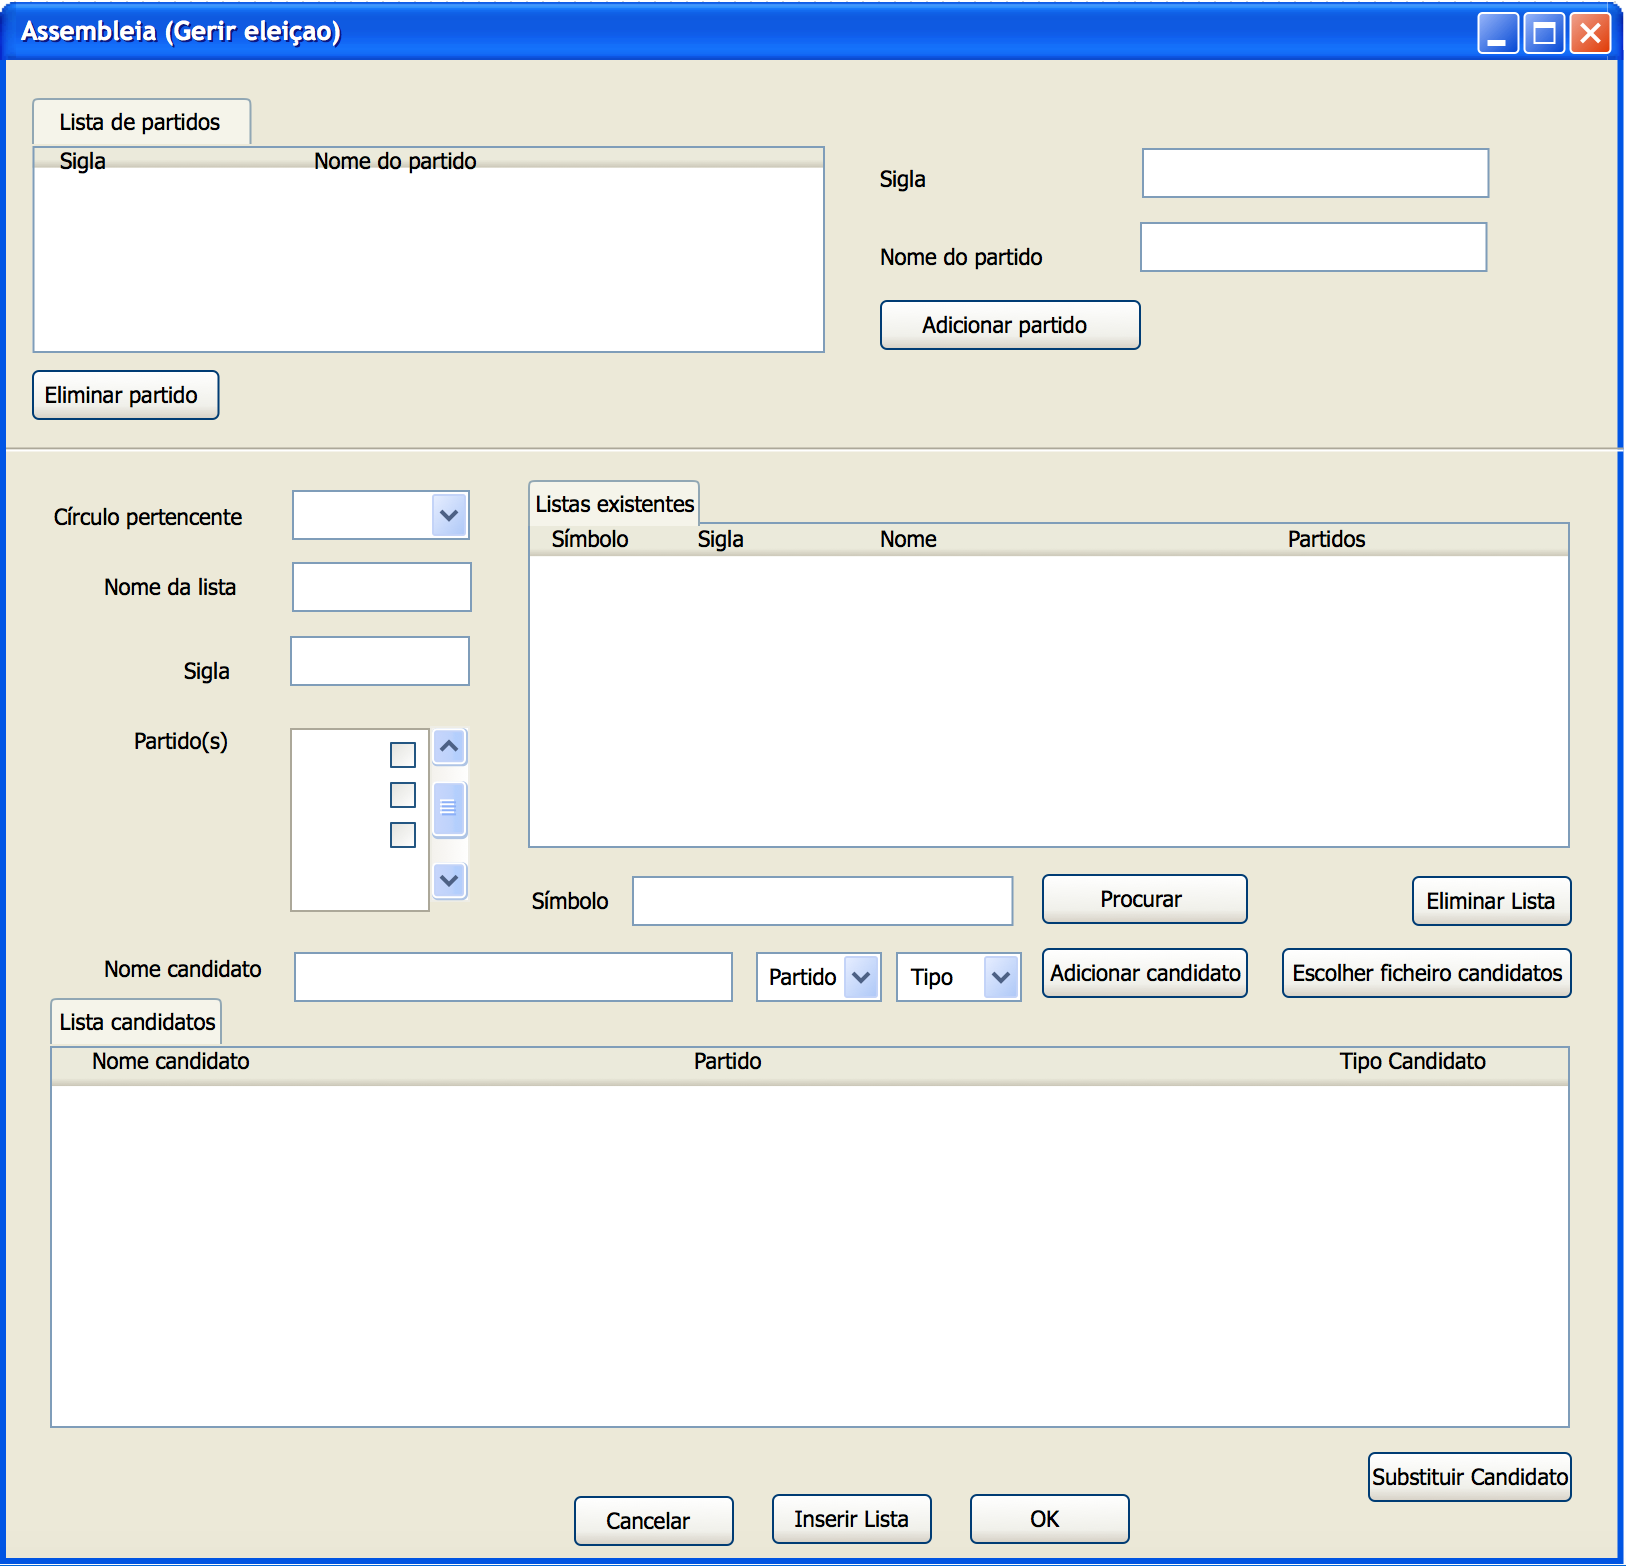
\includegraphics[width=0.7\textwidth]{media/mockup/GerirAR.png}
	 \caption{Gestão de eleições da Assembleia da República.}
\end{center}
\end{figure}
\newpage

\subsubsection{Gerir Eleições da Presidência da República}
Para a gestão das eleições da presidência da república a janela apresentada como os candidatos são a nível nacional, não é necessário a gestão a nível de círculos. A janela permite adicionar um novo candidato inserindo o seu nome e uma foto para ser apresentada, caso o administrador pretenda remover um candidato também deverá ser feito nesta janela.
\begin{figure}[h]
\begin{center}
	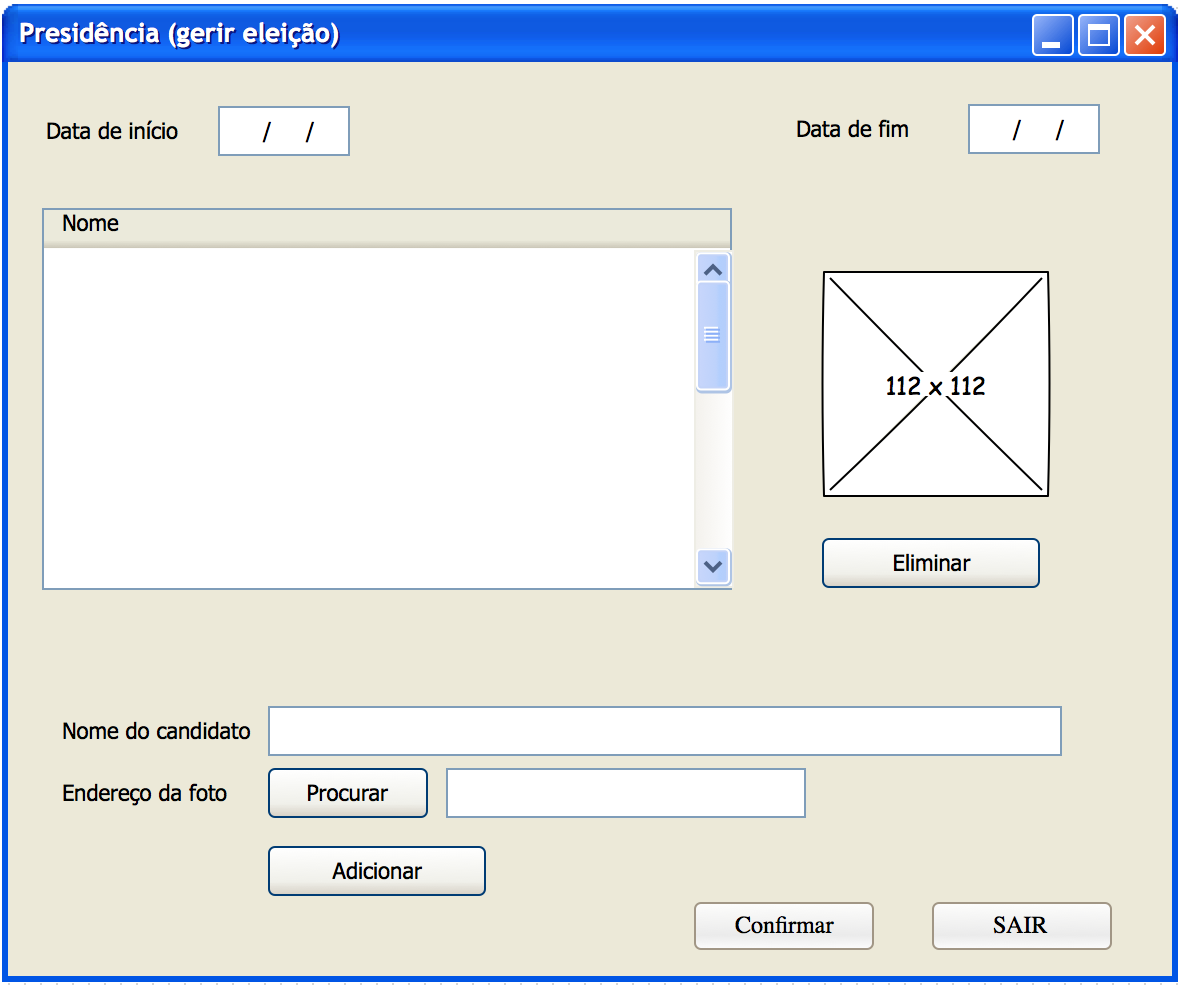
\includegraphics[width=0.5\textwidth]{media/mockup/PRGerir.png}
	 \caption{Gestão de eleições da Presidência da República.}
\end{center}
\end{figure}

\begin{figure}[h]
\begin{center}
	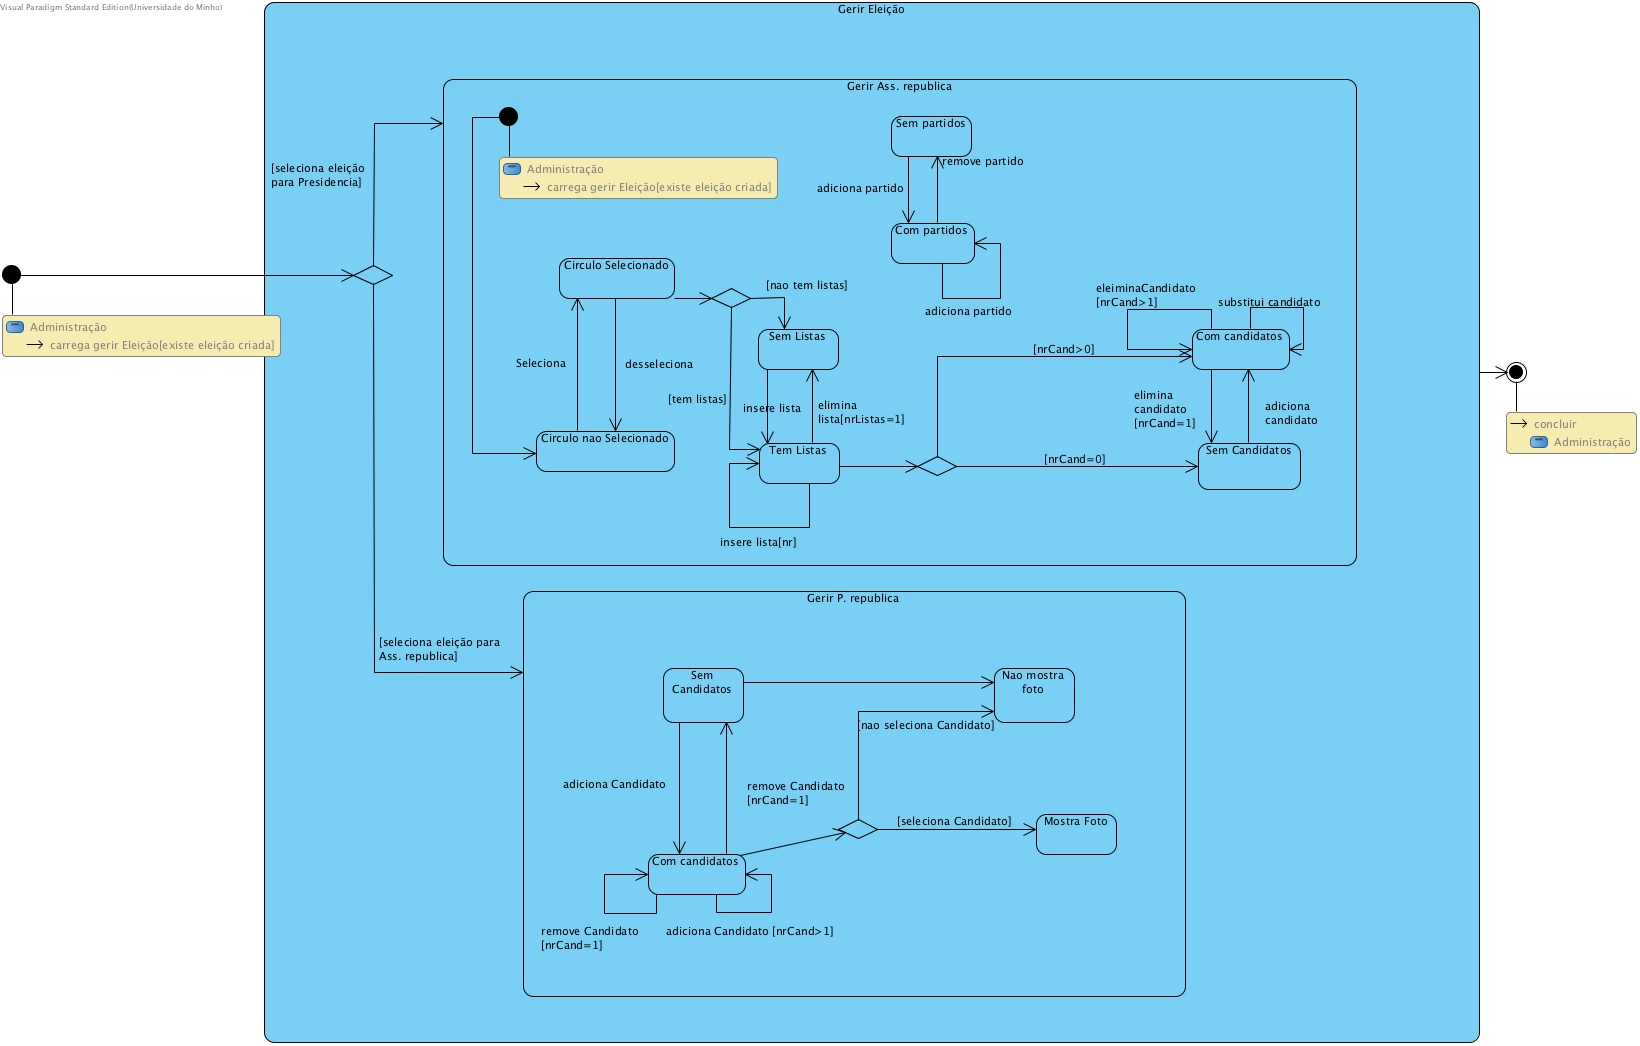
\includegraphics[width=0.5\textwidth]{media/MaqEst/m_GerirEleicao.jpg}
	 \caption{Maquina de estado das janela de Gestão de eleições AR e PR}
\end{center}
\end{figure}

\newpage
\subsubsection{Inserção do Caderno de Recenseamento}

A Inserção do Caderno de Recenseamento é feita com base num ficheiro. Após a inserção é possível visualizar o numero de eleitores do círculo bem como o nome de cada um e o respetivo número de identificação.
\begin{figure}[h]
\begin{center}
	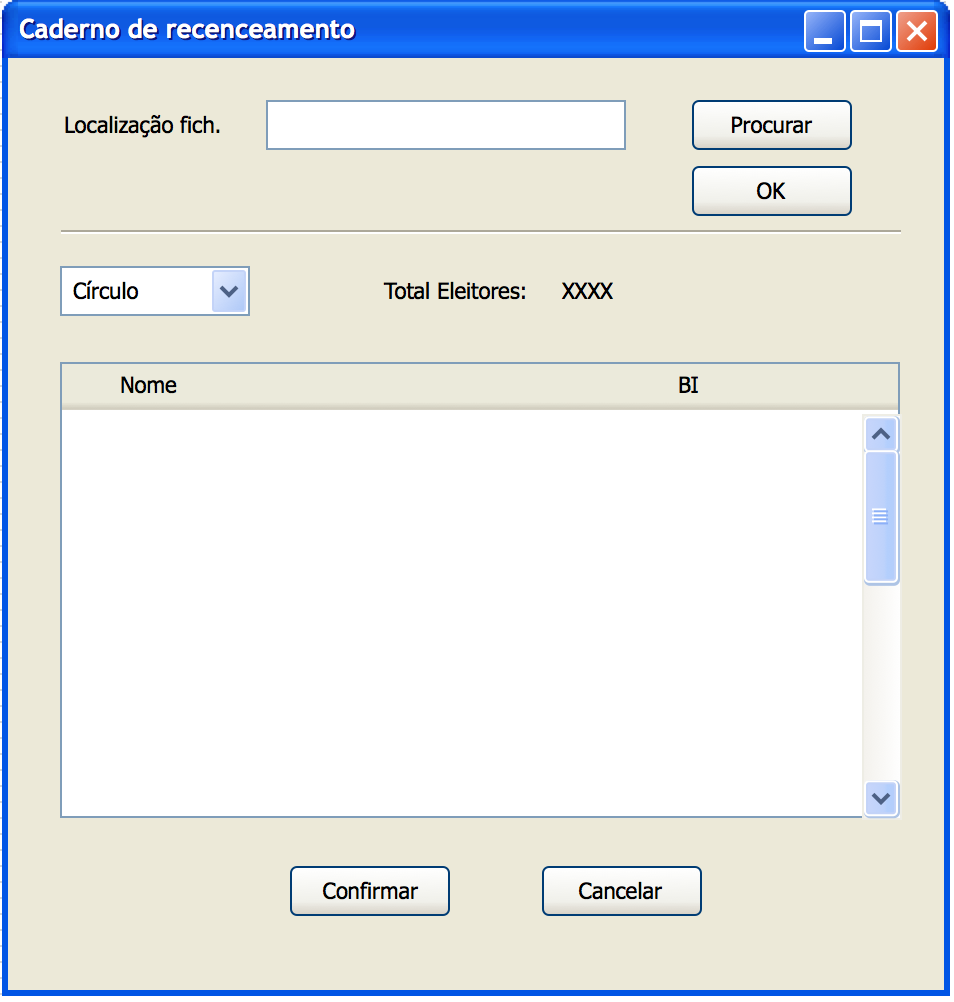
\includegraphics[width=0.4\textwidth]{media/mockup/CR.png}
	 \caption{Inserção do Caderno de Recenseamento.}
\end{center}
\end{figure}

\newpage
\subsection{Janela Principal do eleitor}

Se os dados de login estiverem corretos e forem referentes a um eleitor, aparecerá uma janela de eleitor, onde contém informações sobre o nome deste, o tipo de eleição que está a decorrer, a data de início e de fim, bem como o histórico de eleições já efetuadas.
\indent O utilizador tem a opção de votar para a eleição que está a decorrer, e também de analisar os resultados das eleições que já haviam decorrido.

\begin{figure}[h]
\begin{center}
	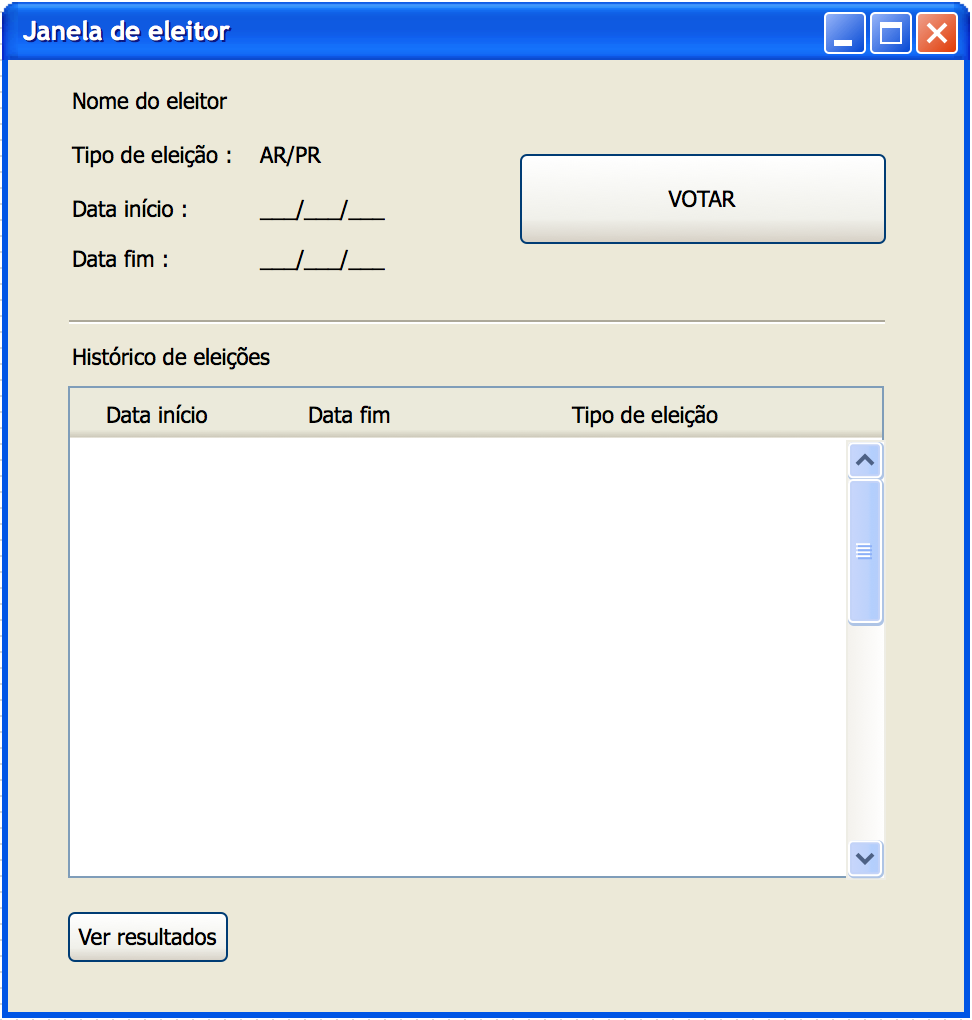
\includegraphics[width=0.5\textwidth]{media/mockup/MainEleitor.png}
	 \caption{Janela Principal do eleitor}
\end{center}
\end{figure}

\begin{figure}[h]
\begin{center}
	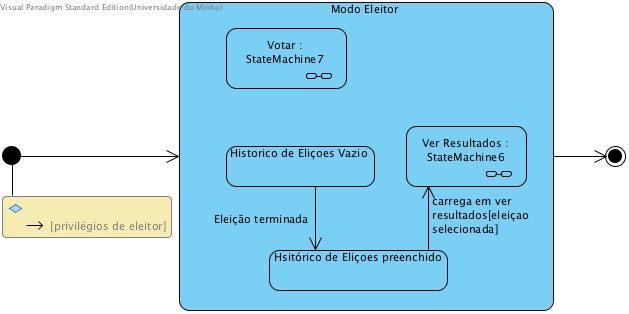
\includegraphics[width=0.5\textwidth]{media/MaqEst/m_modoEleitor.jpg}
	 \caption{Maquina de estado do modo eleitor}
\end{center}
\end{figure}

\newpage
\subsubsection{Boletim de voto}
Caso o eleitor opte por votar, é-lhe apresentada uma janela que corresponde ao boletim de voto. Ao passar o cursor pelas opções, é apresentada à direita uma imagem representativa do partido. Esta janela contém uma lista de opções de votação, na qual cabe ao eleitor escolher uma delas. Caso o utilizador se engane, tem a opção de limpar a sua escolha.

\begin{figure}[h]
\begin{center}
	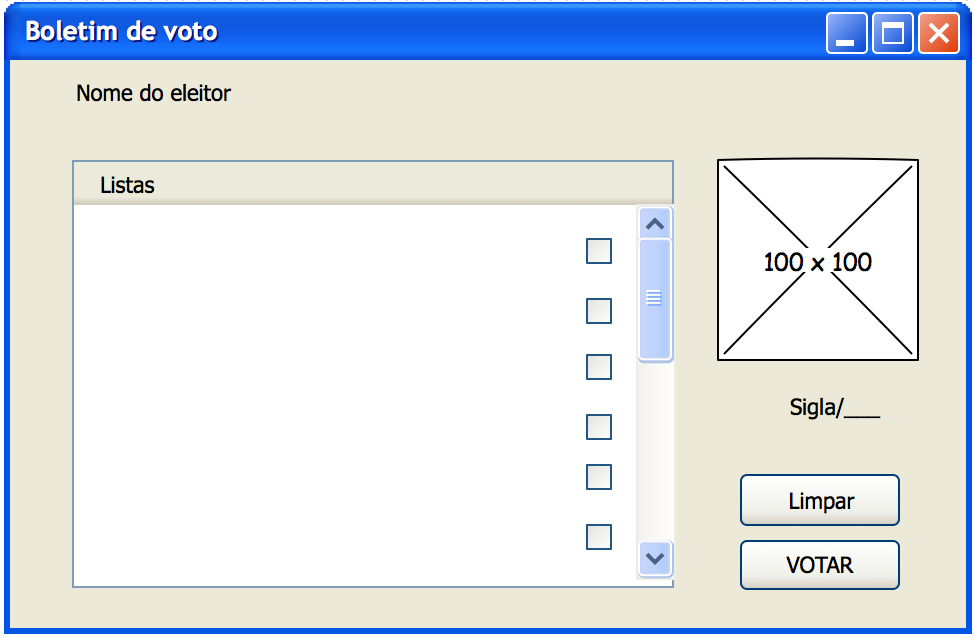
\includegraphics[width=0.6\textwidth]{media/mockup/BoletimVoto.png}
	 \caption{Boletim de Voto}
\end{center}
\end{figure}

\begin{figure}[h]
\begin{center}
	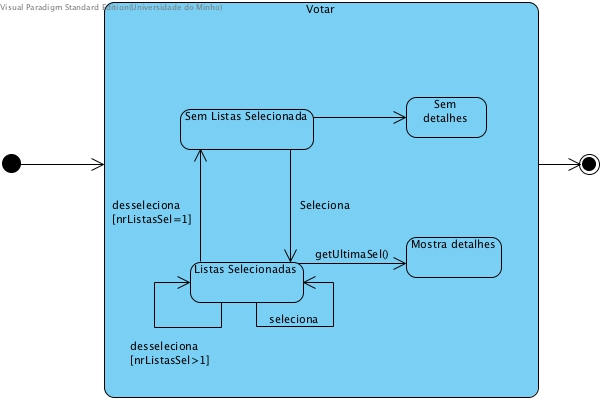
\includegraphics[width=0.6\textwidth]{media/MaqEst/m_Votar.jpg}
	 \caption{Maquina de estado da janela de Voto}
\end{center}
\end{figure}

\newpage
\subsubsection{Resultados Assembleia República}
Caso a eleição presente seja para a Assembleia da República, e o eleitor escolha a opção de ver resultados, é-lhe apresentado uma janela que contém os resultados globais das eleições anteriores (percentagens, lista, mandatos), bem como os resultados divididos por círculos, o que permite ao utilizador analisar detalhadamente e separadamente todas as informações que deseja.

\begin{figure}[h]
\begin{center}
	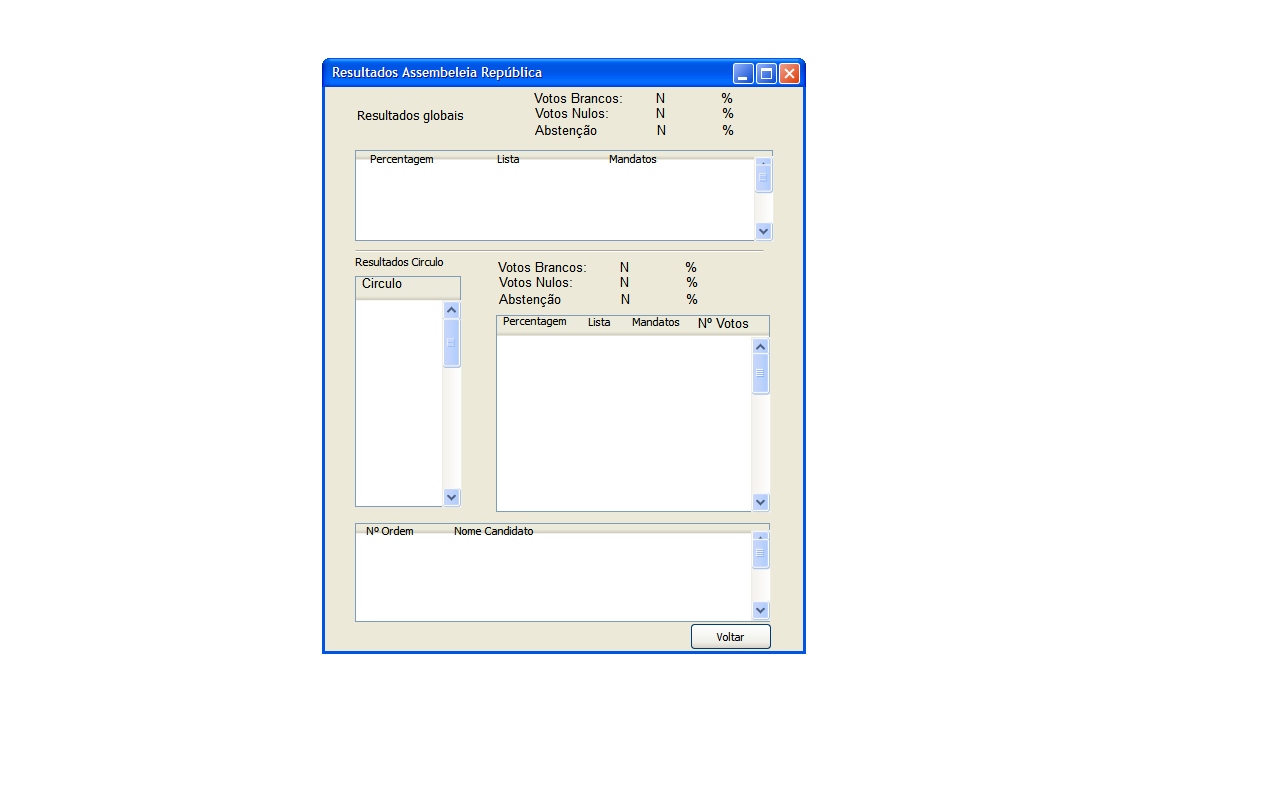
\includegraphics[width=1.3\textwidth]{media/mockup/ver_resultados_ar.png}
	 \caption{Resultados da Assembleia da República}
\end{center}
\end{figure}

\newpage
\subsubsection{Resultados Presidência República}
Caso a eleição presente seja para a Presidência da República, e o eleitor escolha a opção de ver resultados, é-lhe apresentado uma janela idêntica à anterior, mas desta vez sem mandatos.

\begin{figure}[h]
\begin{center}
	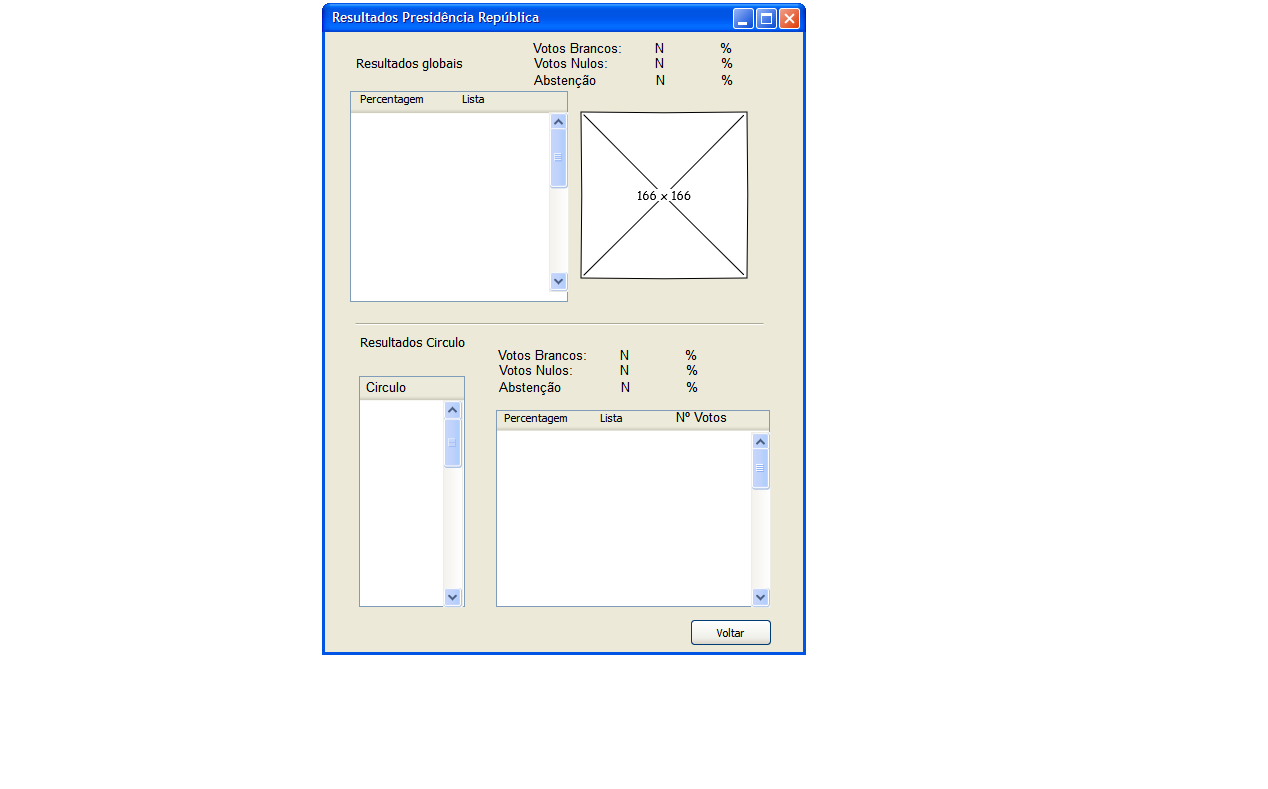
\includegraphics[width=1.3\textwidth]{media/mockup/ver_resultados_pr.png}
	 \caption{Resultados da Presidência da República}
\end{center}
\end{figure}

\begin{figure}[h]
\begin{center}
	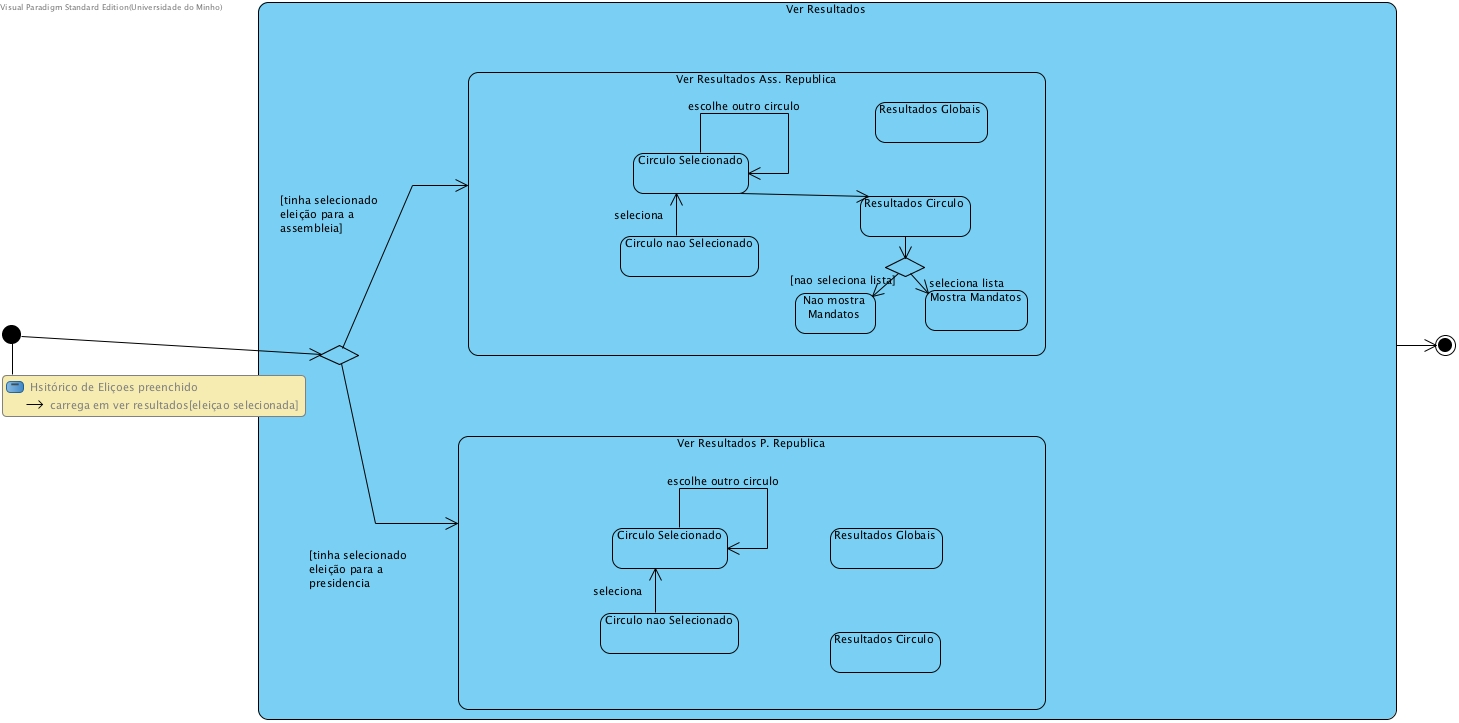
\includegraphics[width=0.8\textwidth]{media/MaqEst/m_VerResultados.jpg}
	 \caption{Maquina de estado da Janela Ver Resultados.}
\end{center}
\end{figure}
\newpage
\clearpage
\section{Conclusão 1ª parte}
Nesta primeira etapa do trabalho prático foram elaborados os Diagramas fundamentais à realização do mesmo. Entre os quais:
\begin{itemize}
\item Modelos de Domínio
\\Nestes modelos identificamos o que a nosso ver seria necessária para as funcionalidades que a nossa aplicação deverá implementar, pondo de parte questões mais burocráticas relacionadas com a administração legal das eleições. 
\\\indent Posto isto focamos maioritariamente na informação que o utilizador necessita aquando e após a realização do voto, ou seja, informação sobre as listas/candidatos, círculos e estatísticas eleitorais.

\item Modelos de Use Case
\\Nestes modelos tentamos identificar as funcionalidades principais que a aplicação deveria ter para com o exterior. Sendo estas divididas em interações com o administrador e o eleitor comum.

\item Diagramas de Sequência de Software
\\Aqui implementámos os use cases previamente definidos. Nesta fase já definimos um pouco a estrutura de classes da nossa aplicação, dividindo a lógica de negócio entre subsistemas. Entre os quais, estão os subsistemas de eleição, círculo (no caso da eleição para a Assembleia da República), lista, candidato (A.R.), e eleitor.

\item Interface e Máquinas de Estado
\\Procurámos desenvolver uma proposta de interface intuitiva e de fácil utilização e navegação, que permitisse oferecer todas as funcionalidades implementadas na aplicação. Para definir o comportamento das janelas e a navegação entre eles, desenvolvemos modelos de máquinas de estado.
\end{itemize}
\indent No decorrer do processo conceptual dos modelos utilizados sentimos dificuldade na junção do modelos elaborados pelos diferentes elementos do grupo pois a quando da sua junção grande parte da vezes o \emph{Visual Paradigm} não deixava, o que levou a ser necessário fazer várias vezes os mesmos diagramas e consequente perda de tempo, precioso noutras partes do desenvolvimento.
\newpage

%%PARTE2
\chapter{Parte 2}
\section{Diagramas Visual Paradigm}
\subsection{Diagramas de Estrutura}
\subsubsection{Diagrama de Classes}
De forma a seguir a metodologia abordada na disciplina, nesta fase, o grupo refinou o Modelo de domínio apresentados na primeira etapa.
De modo a fazer com que este passe a conter linguagem mais próxima dos programadores e para que reflitam de forma total a arquitetura estrutural da aplicação contendo a representação de todas as classes consideradas para a solução.
\\\indent A \emph{Class} principal do da aplicação do Sistema de Gestão de Eleições é a \emph{Class} SGE, 
esta \emph{Class} é a \emph{Facede} para todas as interfaces que desejem utilizar a aplicação a Gestão 
de Eleições devem ``falar'' com esta \emph{Class}.
\\\indent A \emph{Class} \emph{SGE} é a \emph{Class} que sendo a principal trata de toda a gestão da lógica de 
negocio da aplicação controlando todas as restantes classes. Gere também a persistência de dados, para 
isso utiliza as classes do \emph{Package} Data que estabelecem o \emph{ORM} para um base de dados \emph{MySQL}.
\\\emph Esta \emph{Class} de todos os métodos que implementa de modo a proporcionar a comunicação, destacam-se:
\begin{itemize}
\item \emph{confirmarCadernoRecenciamento(Map<Integer, List<Eleitor>> listaEleitores)}:
este método é utilizado para quando quem utiliza o \emph{SGE} confirma que deseja inserir um caderno de  recenseamento que foi lido utilizando o método \emph{lerCadernoRecenciamento(String path)}, este método faz com que toda a informação lida do caderno de recenseamento selecionado se torne persistente, ou seja é passada toda a informação ao \emph{DAO} de eleitores que depois insere na base de dados a informação.
\item \emph{addVoto(Eleição e, Listável lista, Eleitor eleitor)}: Este método encarrega-se de adicionar um voto de um determinado eleitor, numa determinada lista, numa determinada eleição, sendo esta uma eleição da Assembleia da República ou da Presidência da República.
\item \emph{initCirculos()}: Este método é essencial porque é onde se faz a povoação dos círculos. Para cada SGE o valor dos círculos vai ser igual, porque existe sempre a invocação de \emph{initCirculos()}, que não recebe argumentos, logo os valores vão ser sempre os que foram implementados neste método.
 As implementações de algumas das restantes classes serão apresentadas posteriormente.
\end{itemize}


\begin{figure}[H]
\begin{center}
	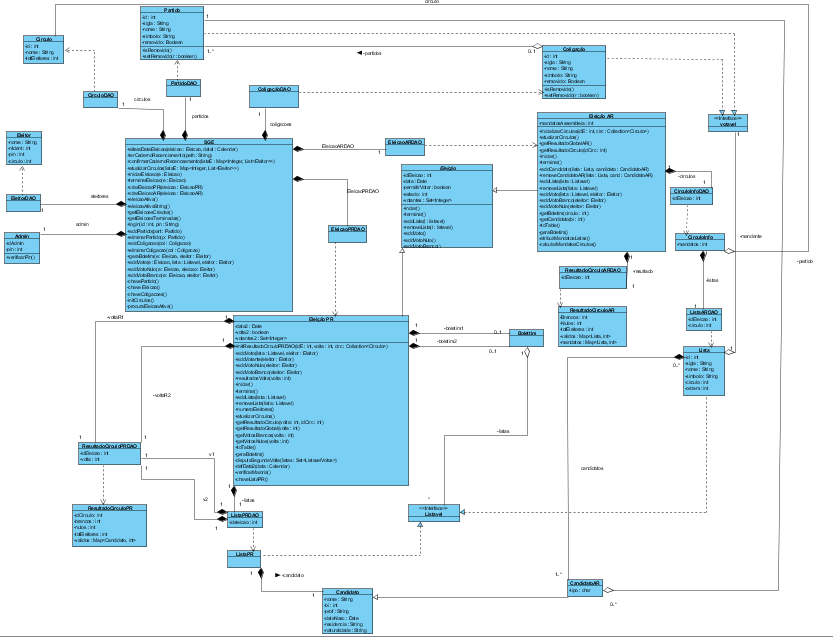
\includegraphics[width=1.23\textwidth]{media/modelodominio/diagramaclass.png}
	 \caption{Diagrama de Classe}
\end{center}
\end{figure}


\subsubsection{Diagrama de Packages}

\begin{figure}[H]
\begin{center}
	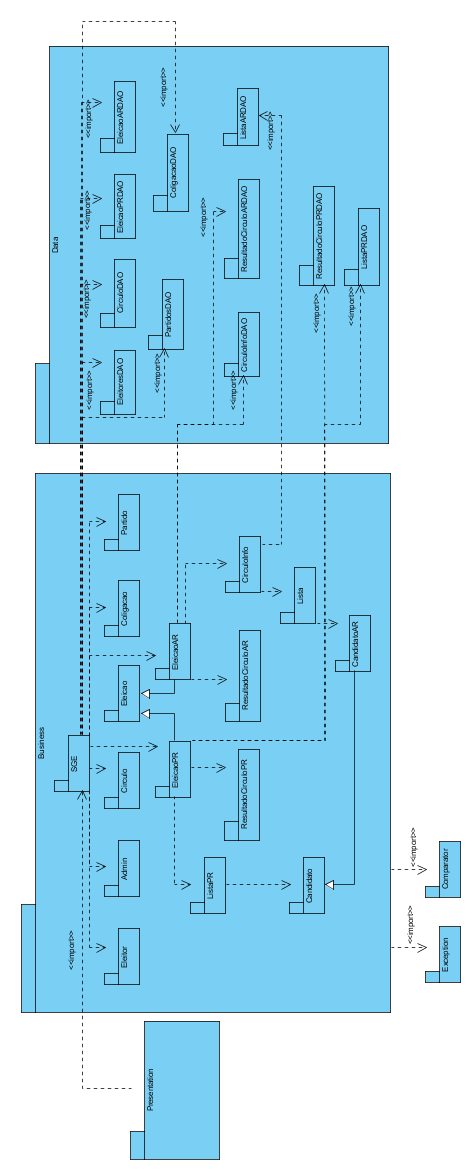
\includegraphics[width=0.5\textwidth]{media/dig_package.png}
	 \caption{Diagrama de Packages}
\end{center}
\end{figure}

Os três principais pacotes definidos são \emph{Presentation}, que trata da apresentação gráfica, em \emph{Java Swing}; \emph{Business}, que contém toda a lógica de negócio; e \emph{Data}, responsável pela ligação à base de dados. A camada de apresentação comunica com a camada de lógica de negócio a partir da classe \emph{SGE} (Sistema de Gestão de Eleições), que desempenha a função de \emph{facade}. Não existe qualquer tipo de comunicação feita diretamente entre a camada de apresentação e a camada de dados.
 A comunicação entre o \emph{package Business} e a persistência de Dados é feita recorrendo às várias classes \emph{DAO} implementadas no \emph{Package} \emph{Data}, que comunicam com a base de dados \emph{MySQL}.
 

\subsubsection{Diagrama de Instalação}

\begin{figure}[H]
	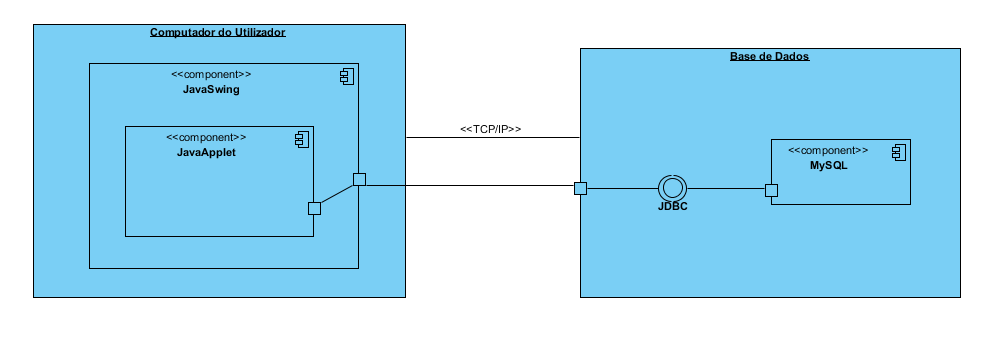
\includegraphics[width=1.2\textwidth]{media/dig_instalacao.png}
	 \caption{Diagrama de Instalação}
\end{figure}

Os dois grandes subsistemas da aplicação desenvolvida são o computador do utilizador e o servidor de base de dados. A comunicação é estabelecida por \emph{TCP/IP}. O programa é uma aplicação Java, e, para a apresentação gráfica ao utilizador, é usado \emph{JavaSwing}. Para ser possível a comunicação entre a aplicação em \emph{Java} e a base de dados \emph{MySQL}, recorre-se à interface \emph{JDBC}\footnote{Java Database Connectivity}.


\newpage
\subsection{Diagramas de Interação}
\subsubsection{Diagrama Sequencia Software}
Devido à elevada extensão destes diagramas, não os vamos apresentar neste relatório, sendo possível consulta-los no projeto do \emph{Visual Paradigm} que foi enviado juntamente com este relatório
\\\indent De forma resumida nesta etapa seguimos o roteiro apresentado nas aulas para a elaboração dos \emph{DSS} utilizando para isso os diagramas apresentados anteriormente que continham a interação entre Subsistemas. Estes subsistemas deram lugar a \emph{Classes} consideradas a quando do detalhe do modelo de domínio para diagrama de classes.
\\\indent A interação entre as \emph{classes} consideradas são também nesta etapa deram lugar a parte da \emph{API} que cada classe deve implementar, ao contrario de simples frases representativas das funcionalidades pretendidas.
\newpage
\section{Código}

\subsection{Classes principais}

O código que desenvolvemos para a criação da nossa aplicação foi desenvolvido em Java, orientada a objetos.
Começamos por criar as classes principais, que achamos que seriam importantes definir.
\begin{itemize}
\item \textbf{Admin}
\\ Contém informação relativa a um administrador do Sistema de gestão de eleições(o seu id e a password), úteis para fazer o login no sistema.
\item \textbf{Boletim}
\\ Contém informação de todas as listas que estão incluídas na eleição relativa ao boletim.
\item \textbf{Candidato}
\\ É a classe relativa a um candidato. A cada candidato diz respeito um número de identificação(bi), uma data de nascimento, um nome, uma profissão, uma residência, uma naturalidade e uma foto.
\item \textbf{CandidatoAR}
\\ CandidatoAR é uma subclasse de candidato, a diferença está no facto de este ter um Partido associado, um caractere que define o tipo de candidato (P:Primário,S:Secundário), e o número de ordem em que ele aparece na lista.
\item \textbf{Circulo}
\\ Cada círculo é composto por um id de Círculo, o nome da região e o número total de eleitores desse circulo em questão.
\item \textbf{CirculoInfo}
\\ A classe CirculoInfo contém um objeto do tipo círculo, e também informação das listas que pertencem àquele círculo, bem como o número de mandatos correspondentes.
\item \textbf{Coligação}
\\ Esta classe implementa uma interface votável, visto que faz parte dos objetos em que é permitido votar. Uma coligação é caracterizada por um elemento de identificação(id), uma sigla, um nome de coligação, um símbolo, a lista de partidos que fazem parte da coligação, e um elemento booleano, que nos diz se essa coligação foi removida do nosso Sistema ou não.
\item \textbf{Eleicao}
\\ Cada eleição é caracterizada por um id, uma data em que é iniciada, um booleano que indica se é permitido votar, um estado de eleição(criada, ativa ou terminada), e um set de todos os votantes que lhe são permitidos votar.
\item \textbf{EleicaoAR}
\\ EleicaoAR é uma subclasse de Eleição. São acrescentados o número de mandatos da Assembleia.
\item \textbf{EleicaoPR}
\\ EleicaoPR é também uma subclasse de Eleição, que contém um booleano que indica se a eleição que está a acontecer é referente à 1ª ou 2ª volta, a data de início, os resultados de eleição relativos a cada círculo, da volta 1 ou da volta 2, uma listagem das listas concorrentes à eleição, e uma listagem de todos os votantes da segunda volta.
\item \textbf{Eleitor}
\\ A cada eleitor diz respeito um nome, o id do Circulo a que pertence, o seu número de identificação e a password que será utilizada para fazer login no sistema.
\item \textbf{Hondt}
\\ È uma classe apenas com metodos de classe que servem para distribuir tanto o número de mandatos da Assembleia pelos respetivos círculos, como o número de mandatos de um determinado círculo pelas respetivas listas.
\item \textbf{Lista}
\\ No nosso sistema, uma lista é caracterizada pelo seu identificador de lista, o círculo a que pertence, o número de ordem que aparece no boletim, a sigla, o nome de lista, o símbolo da lista, o mandante em que é possível votar, e um ArrayList com os candidatos da lista da Assembleia da República.
\item \textbf{ListaPR}
\\ A classe ListaPR implementa, tal como a classe Lista, uma interface Listável, que faz com que estas listas possam ser listáveis. Uma ListaPR (Presidência da República) é caracterizada pelo seu identificador de listaPR, o id da eleição a decorrer, um booleano que traduz o número da volta da eleição, ordem 1 e 2 (ordem em que aparecem no Boletim(tanto na volta 1 como na volta 2)), e o candidato à Presidência da República.
\item \textbf{ListavelVotos}
\\ A classe ListavelVotos é utiizada para uma determinada lista armazenar o número de votos numa eleição.
\item \textbf{Partido}
\\ A classe partido pertence também ao grupo de classes que implementa a interface Votável, e é caracterizada pelo seu id de Partido, a sigla, o nome de Partido, o símbolo, e um booleano a indicar se o Partido já foi removido ou não do sistema.
\item \textbf{ResultadoCirculoAR}
\\ ResultadoCirculoAR foi usada para representar os resultados referentes a um determinado círculo de uma eleição da Assembleia da República. Informação essa que se traduz no número total de eleitores, e nos votos atribuidos a esse círculo.
\item \textbf{ResultadoCirculoPR}
\\ ResultadoCirculoPR foi usada para representar os resultados referentes a um determinado círculo de uma eleição da Presidência da República. Informação essa que se traduz no número total de eleitores, e nos votos atribuidos nesse círculo.
\item \textbf{ResultadoGlobalAR} e \textbf{ResultadoGlobalPR}
\\ As classes ResultadoGlobalAR e ResultadoGlobalPR foram criadas de maneira a armazenar os resultados e dados relativos às eleições, mas desta vez de todos os círculos.
\item \textbf{VotavelVotos}
\\ Criamos a Class VotavelVotos de maneira a agrupar o número dos votos de um determinado Votável(Partido ou Coligação).
\item \textbf{SGE}
\\ SGE é a nossa classe principal, onde estão incluídos os métodos relevantes, que serão utilizados na nossa interface.
Faz-se a declaração das classes principais, e dos DAOs(falaremos destes posteriormente).
\newpage
\end{itemize}
\subsection{DAOs}
Para a realização deste projeto, construímos uma base de dados relacional em \emph{MySQL} para armazenar toda a informação necessária para meter o Sistema de Eleições a correr. Para o nosso programa aceder a essa informação, nós criamos as classes \emph{DAO}, que nos forneciam métodos de acesso à base de dados.
\\\indent Poderíamos abordar todos os \emph{DAOs} independentemente, mas a verdade é que são quase todos 
muito semelhantes. Cada método visível para o exterior destas classe solicita sempre um Conceção à base de Dados, este pedido é feito à classe \emph{Connector}, podendo este conetor estar configurado com \emph{AutoCommit} ou não dependendo do tipo de operações pretendidas.
\\\indent São também definidos métodos auxiliares alguns \emph{Private} e outros \emph{Protected} que executam as \emph{queries} à base de dados, contêm \emph{PreparedStatements} por questões de segurança contra \emph{SQL injection}. A criação destes métodos deve-se à tentativa de minimizar as conceções simultâneas à Base de Dados.
\subsubsection{Estratégias utilizadas para otimizar os DAOs e Base de Dados}
Decidimos, que na base de dados, na tabela referente às listas candidatas a uma Eleição de assembleia da República continha o id de um partido e o id de uma coligação, devendo um deles ser \emph{null}. Caso o \emph{idPartido} seja diferente de \emph{null}, o \emph{idColigação} deverá ser \emph{null}, e vice-versa, porque não existe uma lista que tenha um partido e uma coligação a concorrer à mesma eleição.
\\\indent Sentimos tambem a necessidade de criar uma tabela para cada tipo de eleição resultando assim em dois \emph{DAOs}, o  \emph{EleicaoDAOAR} e \emph{EleicaoDAOPR}, esta divisão deve-se a facilitar a representação dos objetos na base de dados. Apesar desta divisão existe também uma tabela Eleição que contem os campos comuns aos dois tipos de eleição, cujo os dados são tratados pelos dois \emph{DAO's} referidos. 
\\\indent Não sentimos necessário implementar certos \emph{DAO's}, como por o que trataria da comunicação dos dados dos Candidatos pois tais informações são transferidas de/para a base de dados
noutros \emph{DAO's}. Neste caso, a informação de um candidato é obtida quando se vai buscar 
informação à tabela das listas a que esse candidato pertence.
\\\indent Todos os \emph{DAO's} implementam a interface \emph{Map<K,V>}\footnote{java.util.Map}, como foi sugerido nas aulas, devido a inicialmente ser sugerido que a representação de dados fosse feita em \emph{Map}, mas também pelo facto de o modelo relacional ser muito semelhante ao \emph{Map}, sendo que para cada chave obtemos um dado Valor.
\\\indent Algumas entidades presentes na nossa abordagem, na base de dados teriam a necessidade de terem chaves compostas, como por exemplo o ResultadoCirculoAR que a sua chave seria o Id da eleição a que esses resultados pertence e o id do circulo em questão. Posto isto o \emph{DAO} representativo desta classe tem como variável de instância o id da Eleição, sendo a sua chave quando referido apenas o Id do Circulo. 
\\\indent Como referido a cima de forma a reduzir o número de conexões existentes à  base de dados, nos DAOs decidimos criar métodos auxiliares sendo alguns \emph{protected}, de maneira a poderem ser utilizados por outras classes do mesmo \emph{package}, por exemplo o \emph{ListaPRDAO} utiliza métodos de \emph{ResultadoCirculoPRDAO}, um outro exemplo é o método \emph{values()} que utiliza o método \emph{keySet()} e seguidamente múltiplas vezes o método \emph{get()} com todos os valores retornados pelo no \emph{Set}. Estes recebem como argumento uma conexão, e a partilham. Isto resulta numa diminuição significativa do número de conexões à base de Dados, impedindo falhas de sistema inconvenientes, também resulta numa melhor qualidade nas transações pois apenas é utilizada uma conexão e caso alguma operação que seja realizada utilizando esta conexão falhe todas as operações anteriores são desfeitas. Este método faz com que seja muito difícil levar a base de dados a um estado de inconsistência, permitindo assim maior fidelidade na aplicação.\footnote{*Em anexo encontra-se o modelo lógico da base de dados utilizada.}
\newpage
\subsection{Interface}
Apesar da proposta de interface apresentada anteriormente e de tentarmos manter tais interfaces, durante o desenvolvimento do projeto apercebemos-nos de algumas impossibilidades tecnológicas relativas a alguns aspetos da janelas idealizadas. 
\\\indent Por outro lado foram efetuadas alterações a algumas janelas devido à necessidade ou não de introdução de certos dados. Também existiram alterações devido à elevada complexidade das interfaces apresentas, um dos grandes problemas que nos deparamos na execução do projeto, houve necessidade de simplificar.
O programa inicia com uma janela de login.
\begin{figure}[H]
\begin{center}
	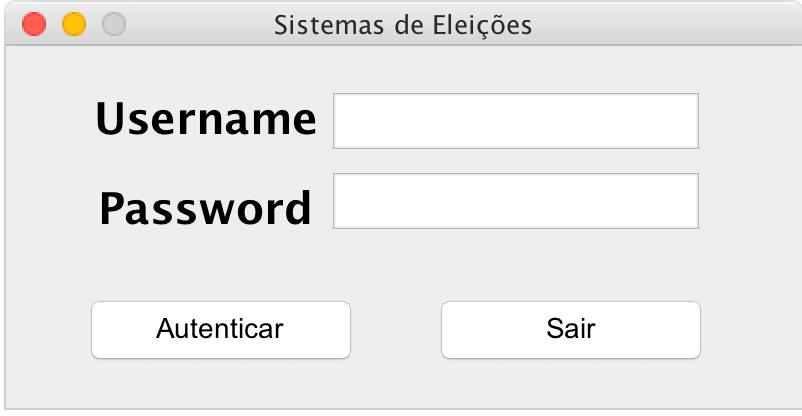
\includegraphics[width=0.45\textwidth]{media/img_interface/img2.jpg}
	 \caption{Login}
\end{center}
\end{figure}
Caso seja um eleitor a fazer o login, é-lhe apresentado a seguinte janela:
\begin{figure}[H]
\begin{center}
	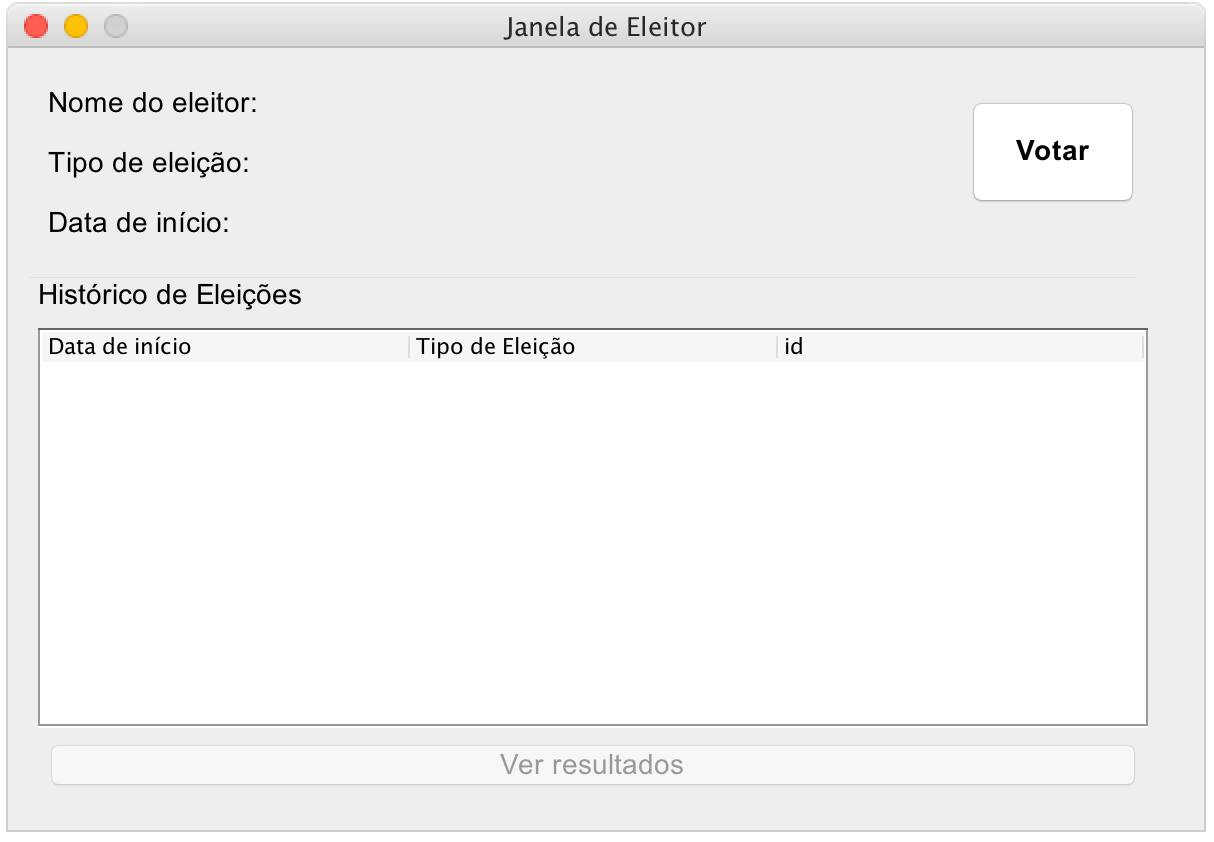
\includegraphics[width=0.8\textwidth]{media/img_interface/img10.jpg}
	 \caption{Janela de eleitor}
\end{center}
\end{figure}
Nesta janela é permito ao eleitor votar numa lista, ou ver os resultados tanto da Assembleia da República como da Presidência da República, de eleições que já decorreram.
\begin{figure}[H]
\begin{center}
	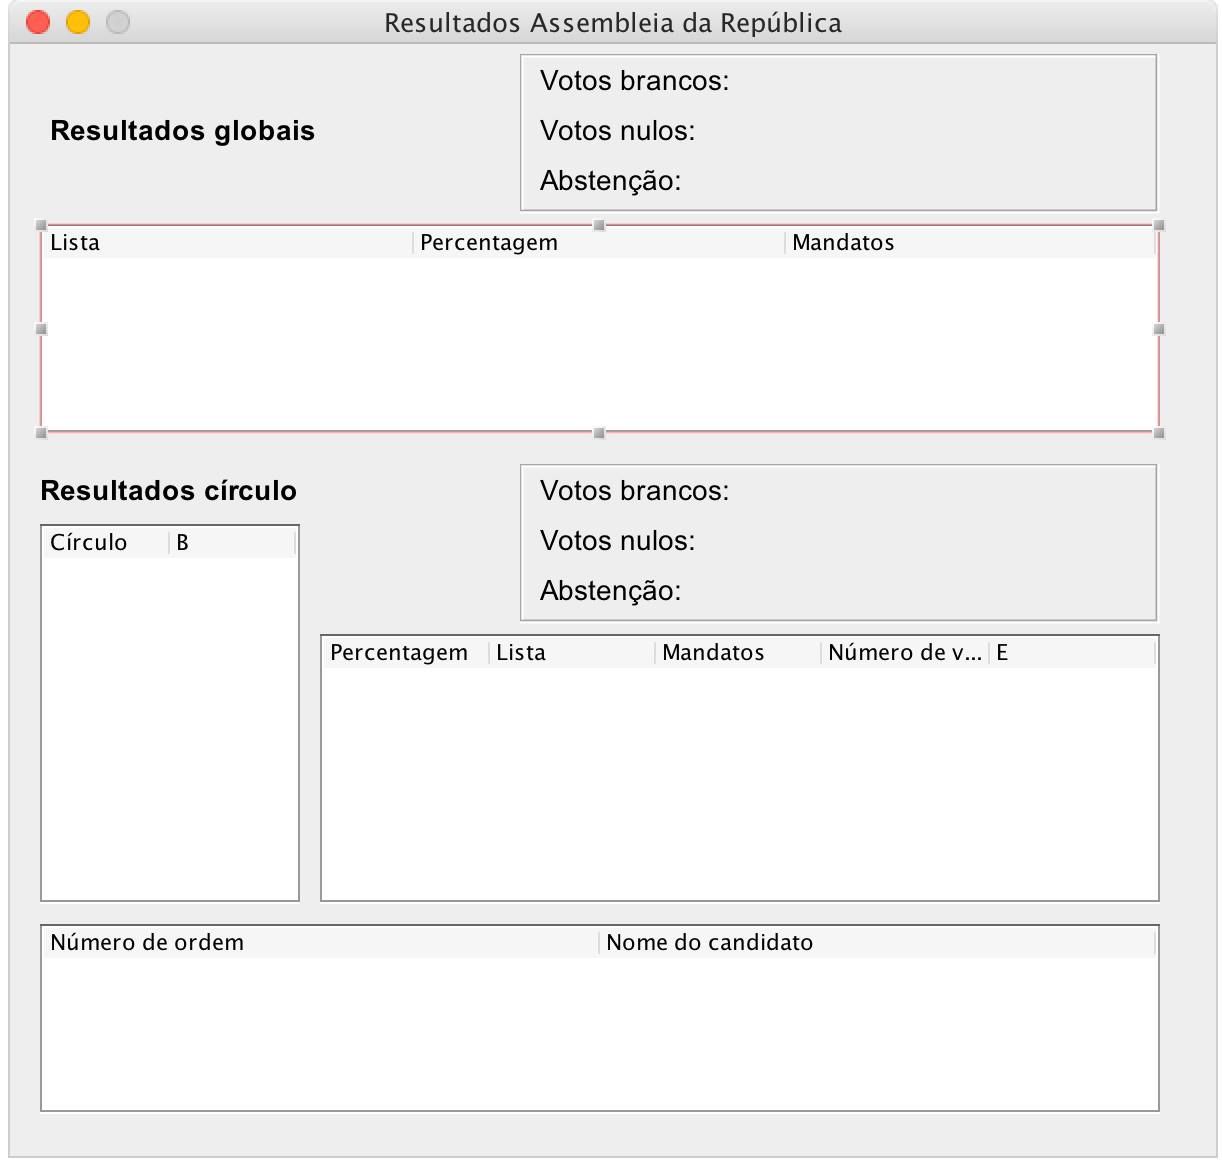
\includegraphics[width=0.5\textwidth]{media/img_interface/img5.jpg}
	 \caption{Resultados da Assembleia da República}
\end{center}
\end{figure}
\begin{figure}[H]
\begin{center}
	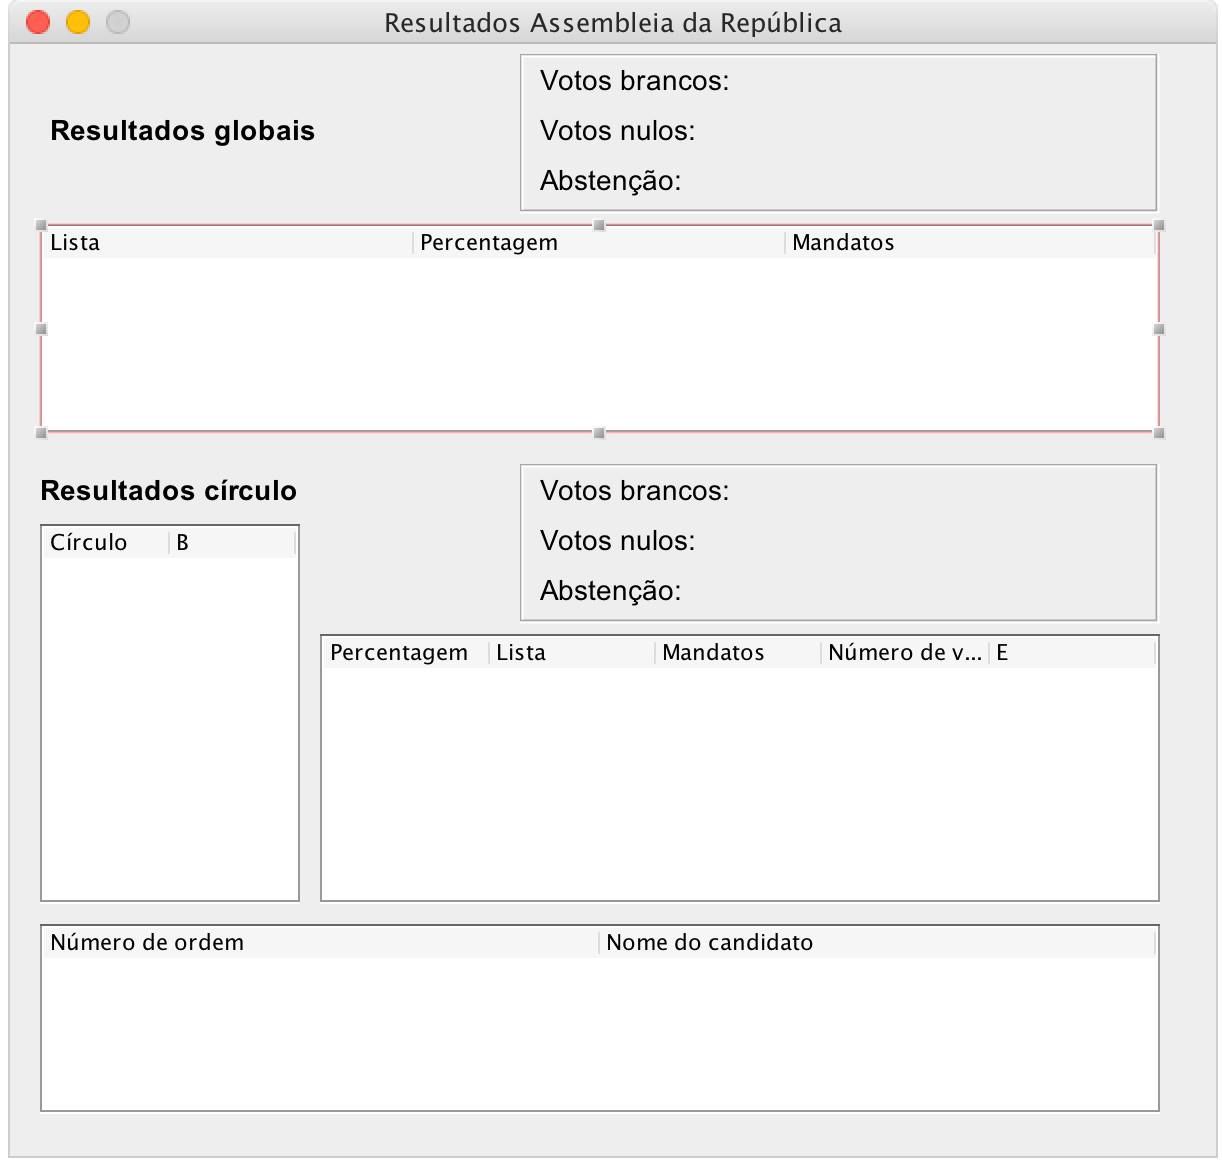
\includegraphics[width=0.5\textwidth]{media/img_interface/img5.jpg}
	 \caption{Resultados na Presidência da República}
\end{center}
\end{figure}
Caso o eleitor escolha votar numa lista, é-lhe apresentado o boletim de voto.
\begin{figure}[H]
\begin{center}
	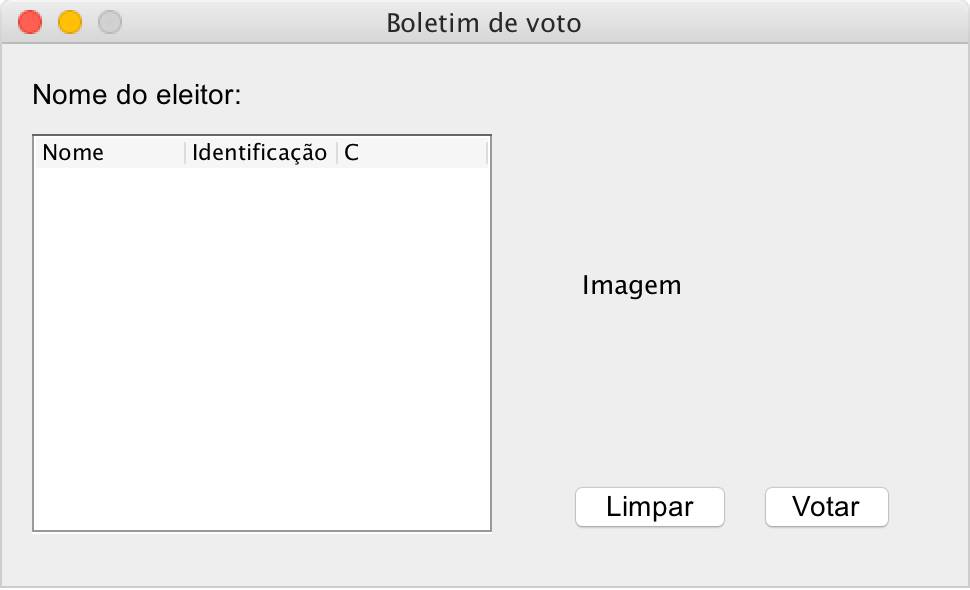
\includegraphics[width=0.5\textwidth]{media/img_interface/img4boletim.jpg}
	 \caption{Boletim de voto}
\end{center}
\end{figure}
Se for um administrador a fazer o login, é-lhe apresentada a seguinte janela:
\begin{figure}[H]
\begin{center}
	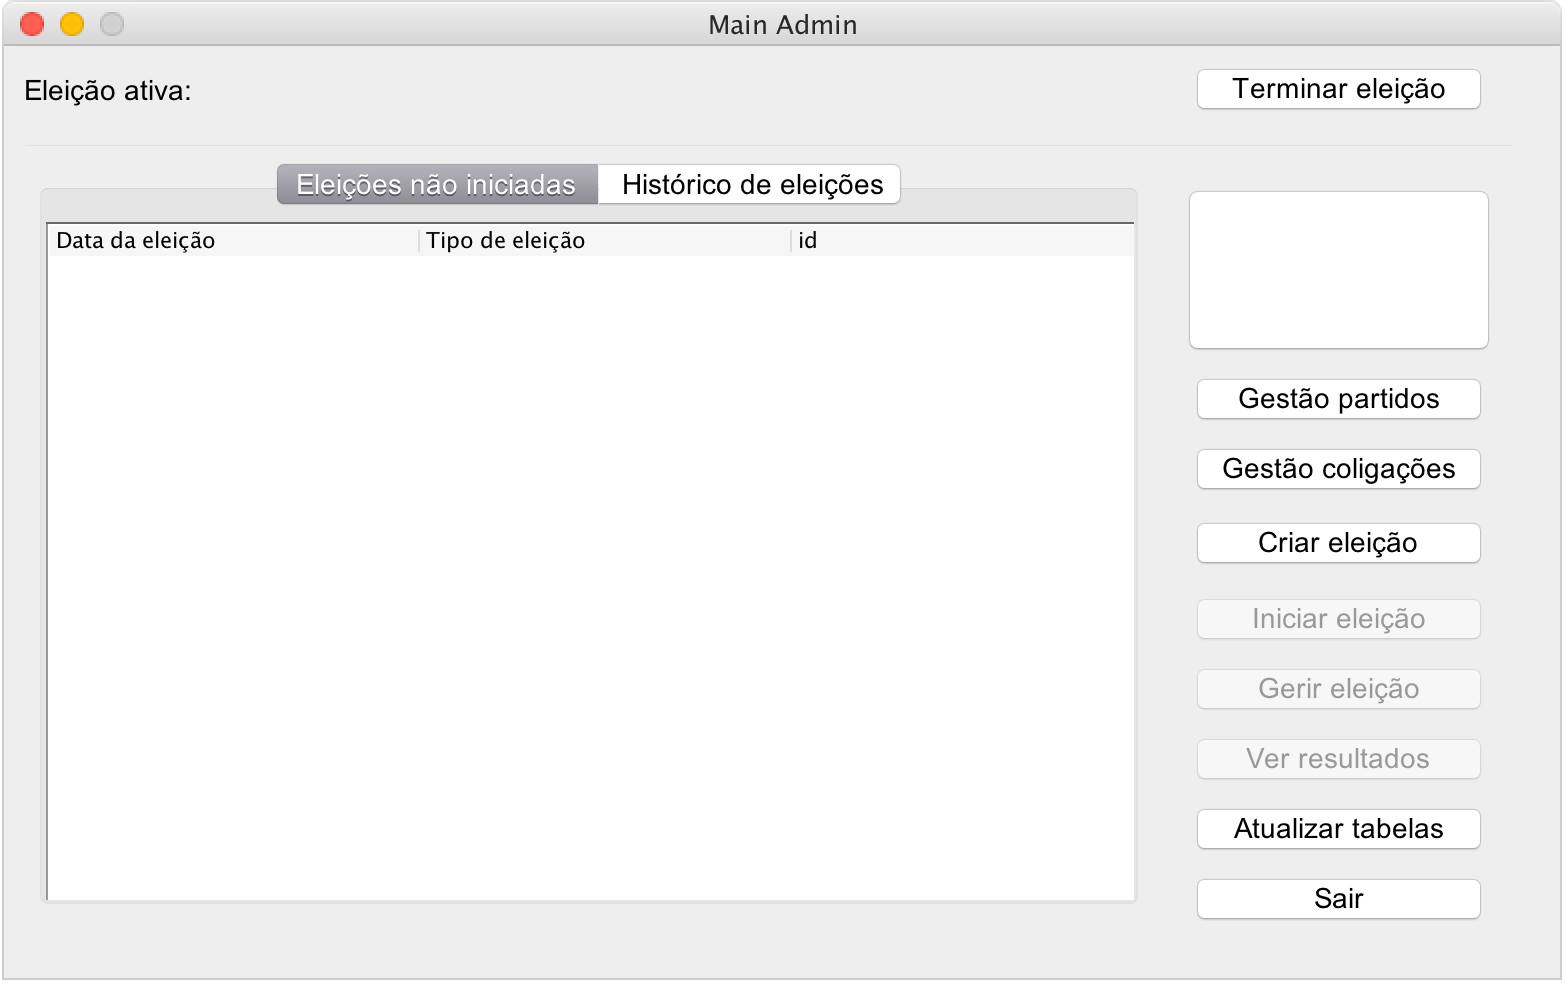
\includegraphics[width=0.5\textwidth]{media/img_interface/img9.jpg}
	 \caption{Main admin}
\end{center}
\end{figure}
O administrador pode optar por fazer a gestão de partidos ou coligações:
\begin{figure}[H]
\begin{center}
	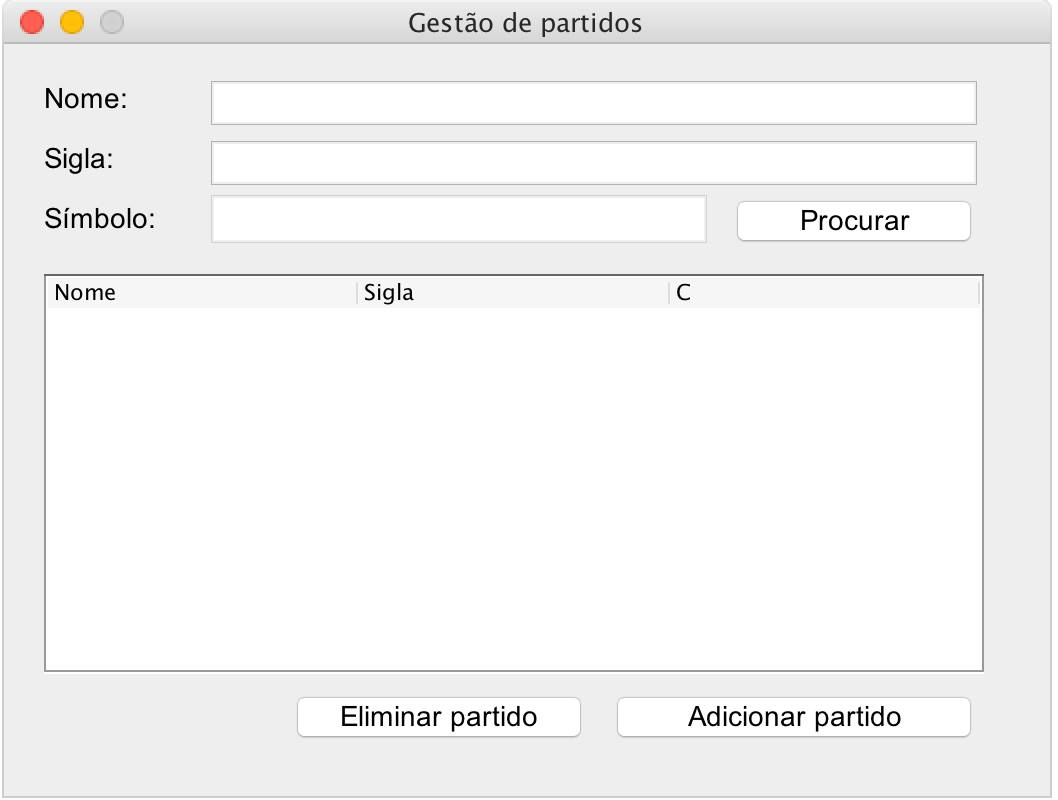
\includegraphics[width=0.5\textwidth]{media/img_interface/img3.jpg}
	 \caption{Gestão de partidos}
\end{center}
\end{figure}

\begin{figure}[H]
\begin{center}
	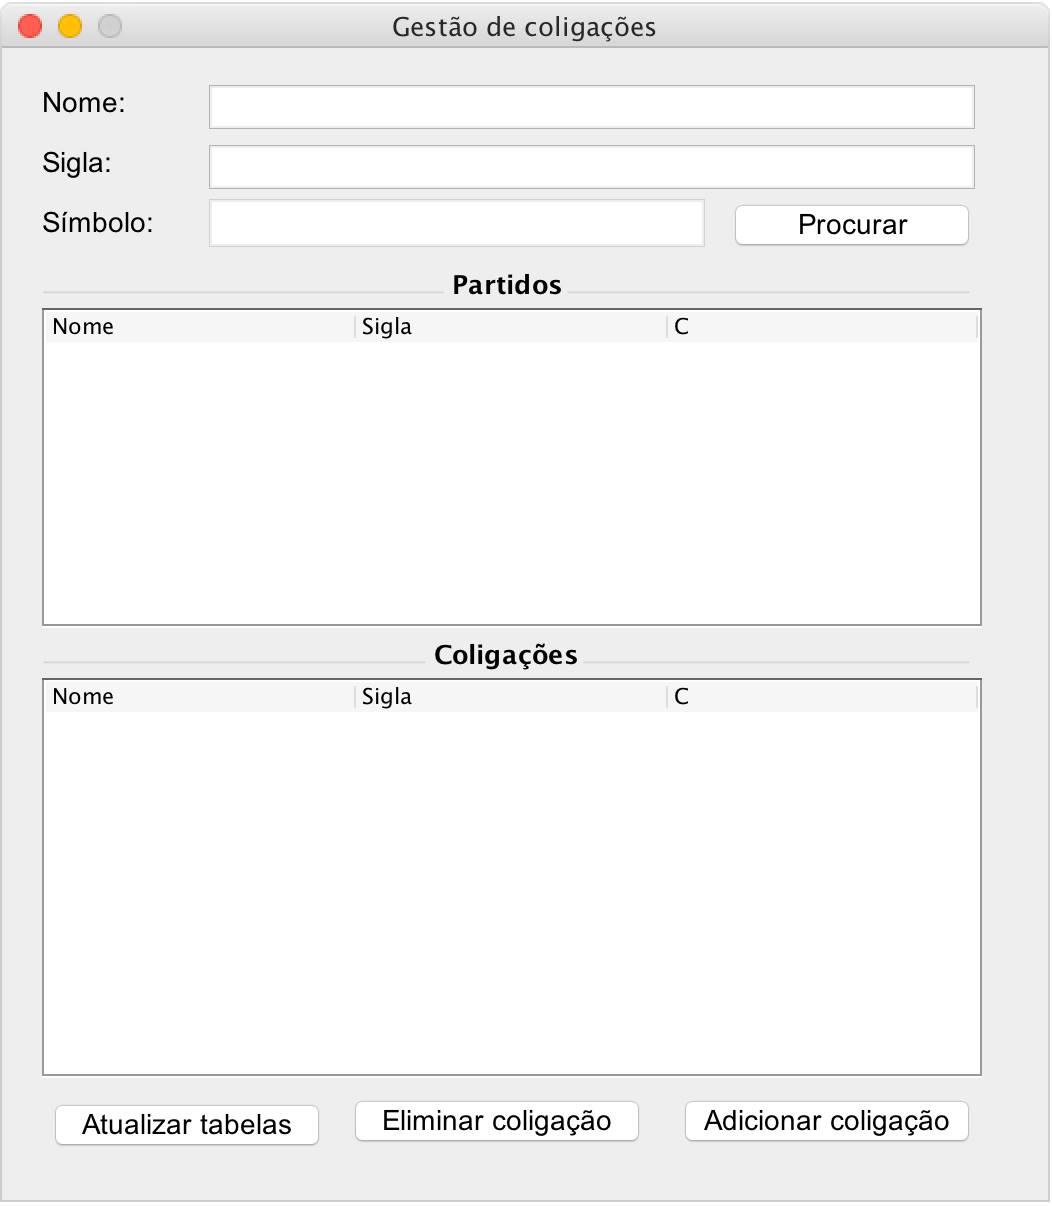
\includegraphics[width=0.5\textwidth]{media/img_interface/img4.jpg}
	 \caption{Gestão de coligações}
\end{center}
\end{figure}
Pode também fazer a inserção dos cadernos de recenseamento:
\begin{figure}[H]
\begin{center}
	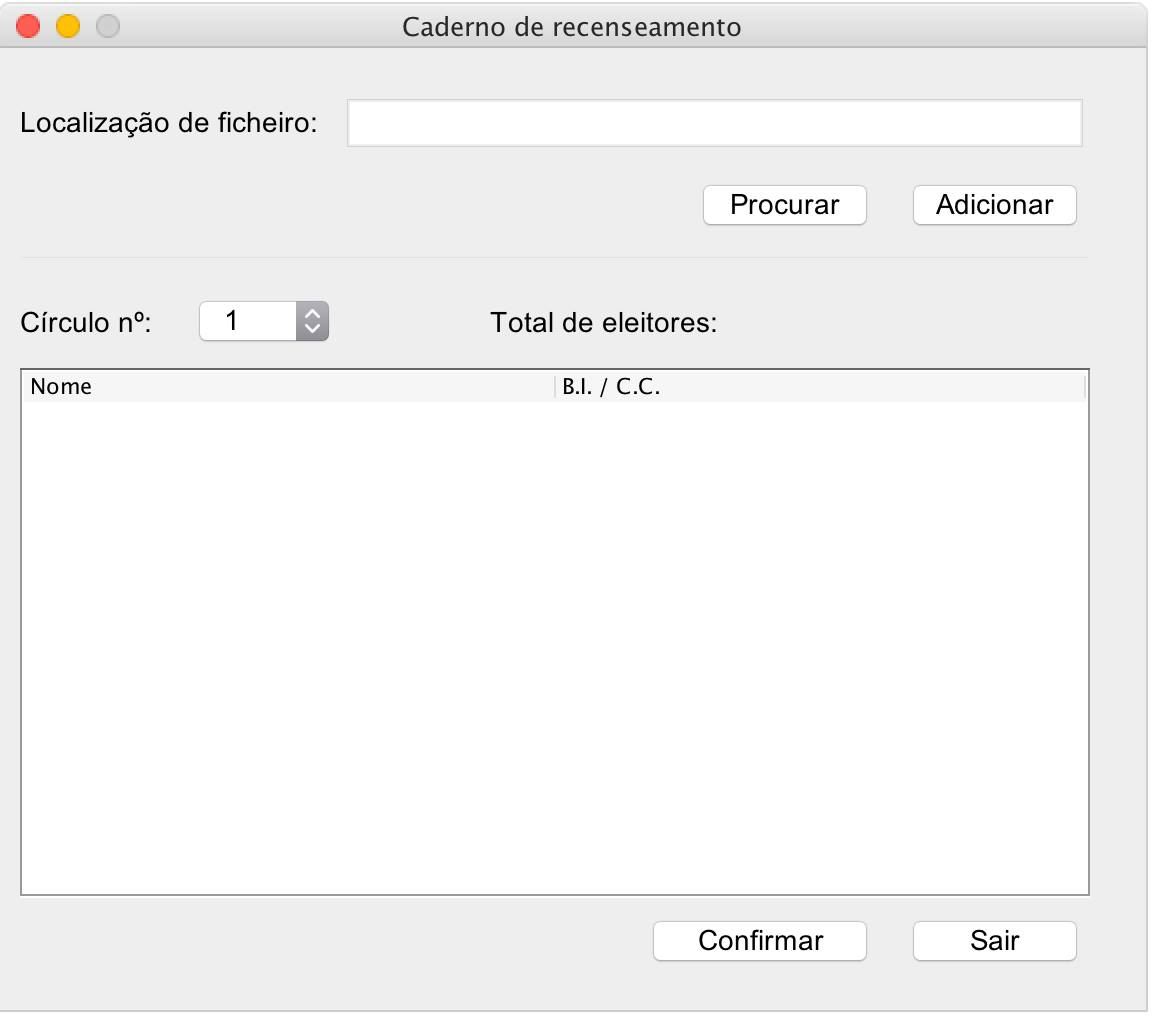
\includegraphics[width=0.5\textwidth]{media/img_interface/img8.jpg}
	 \caption{Inserção dos cadernos de recenseamento}
\end{center}
\end{figure}
O administrador pode criar uma nova eleição:
\begin{figure}[H]
\begin{center}
	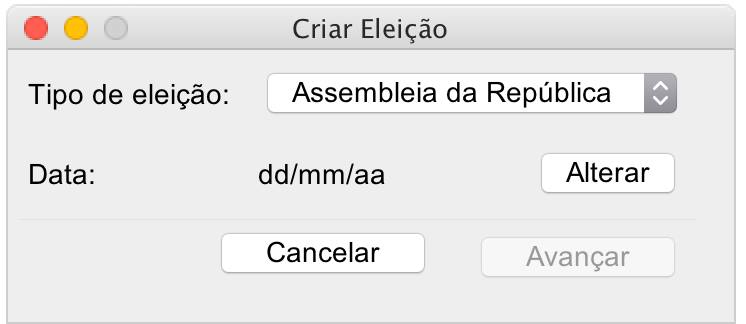
\includegraphics[width=0.5\textwidth]{media/img_interface/img1.jpg}
	 \caption{Criar eleição}
\end{center}
\end{figure}
Caso já tenha sido criada uma eleição, o administrador pode tem a opção de gerir tanto uma eleição da Assembleia como da Presidência da República:
\begin{figure}[H]
\begin{center}
	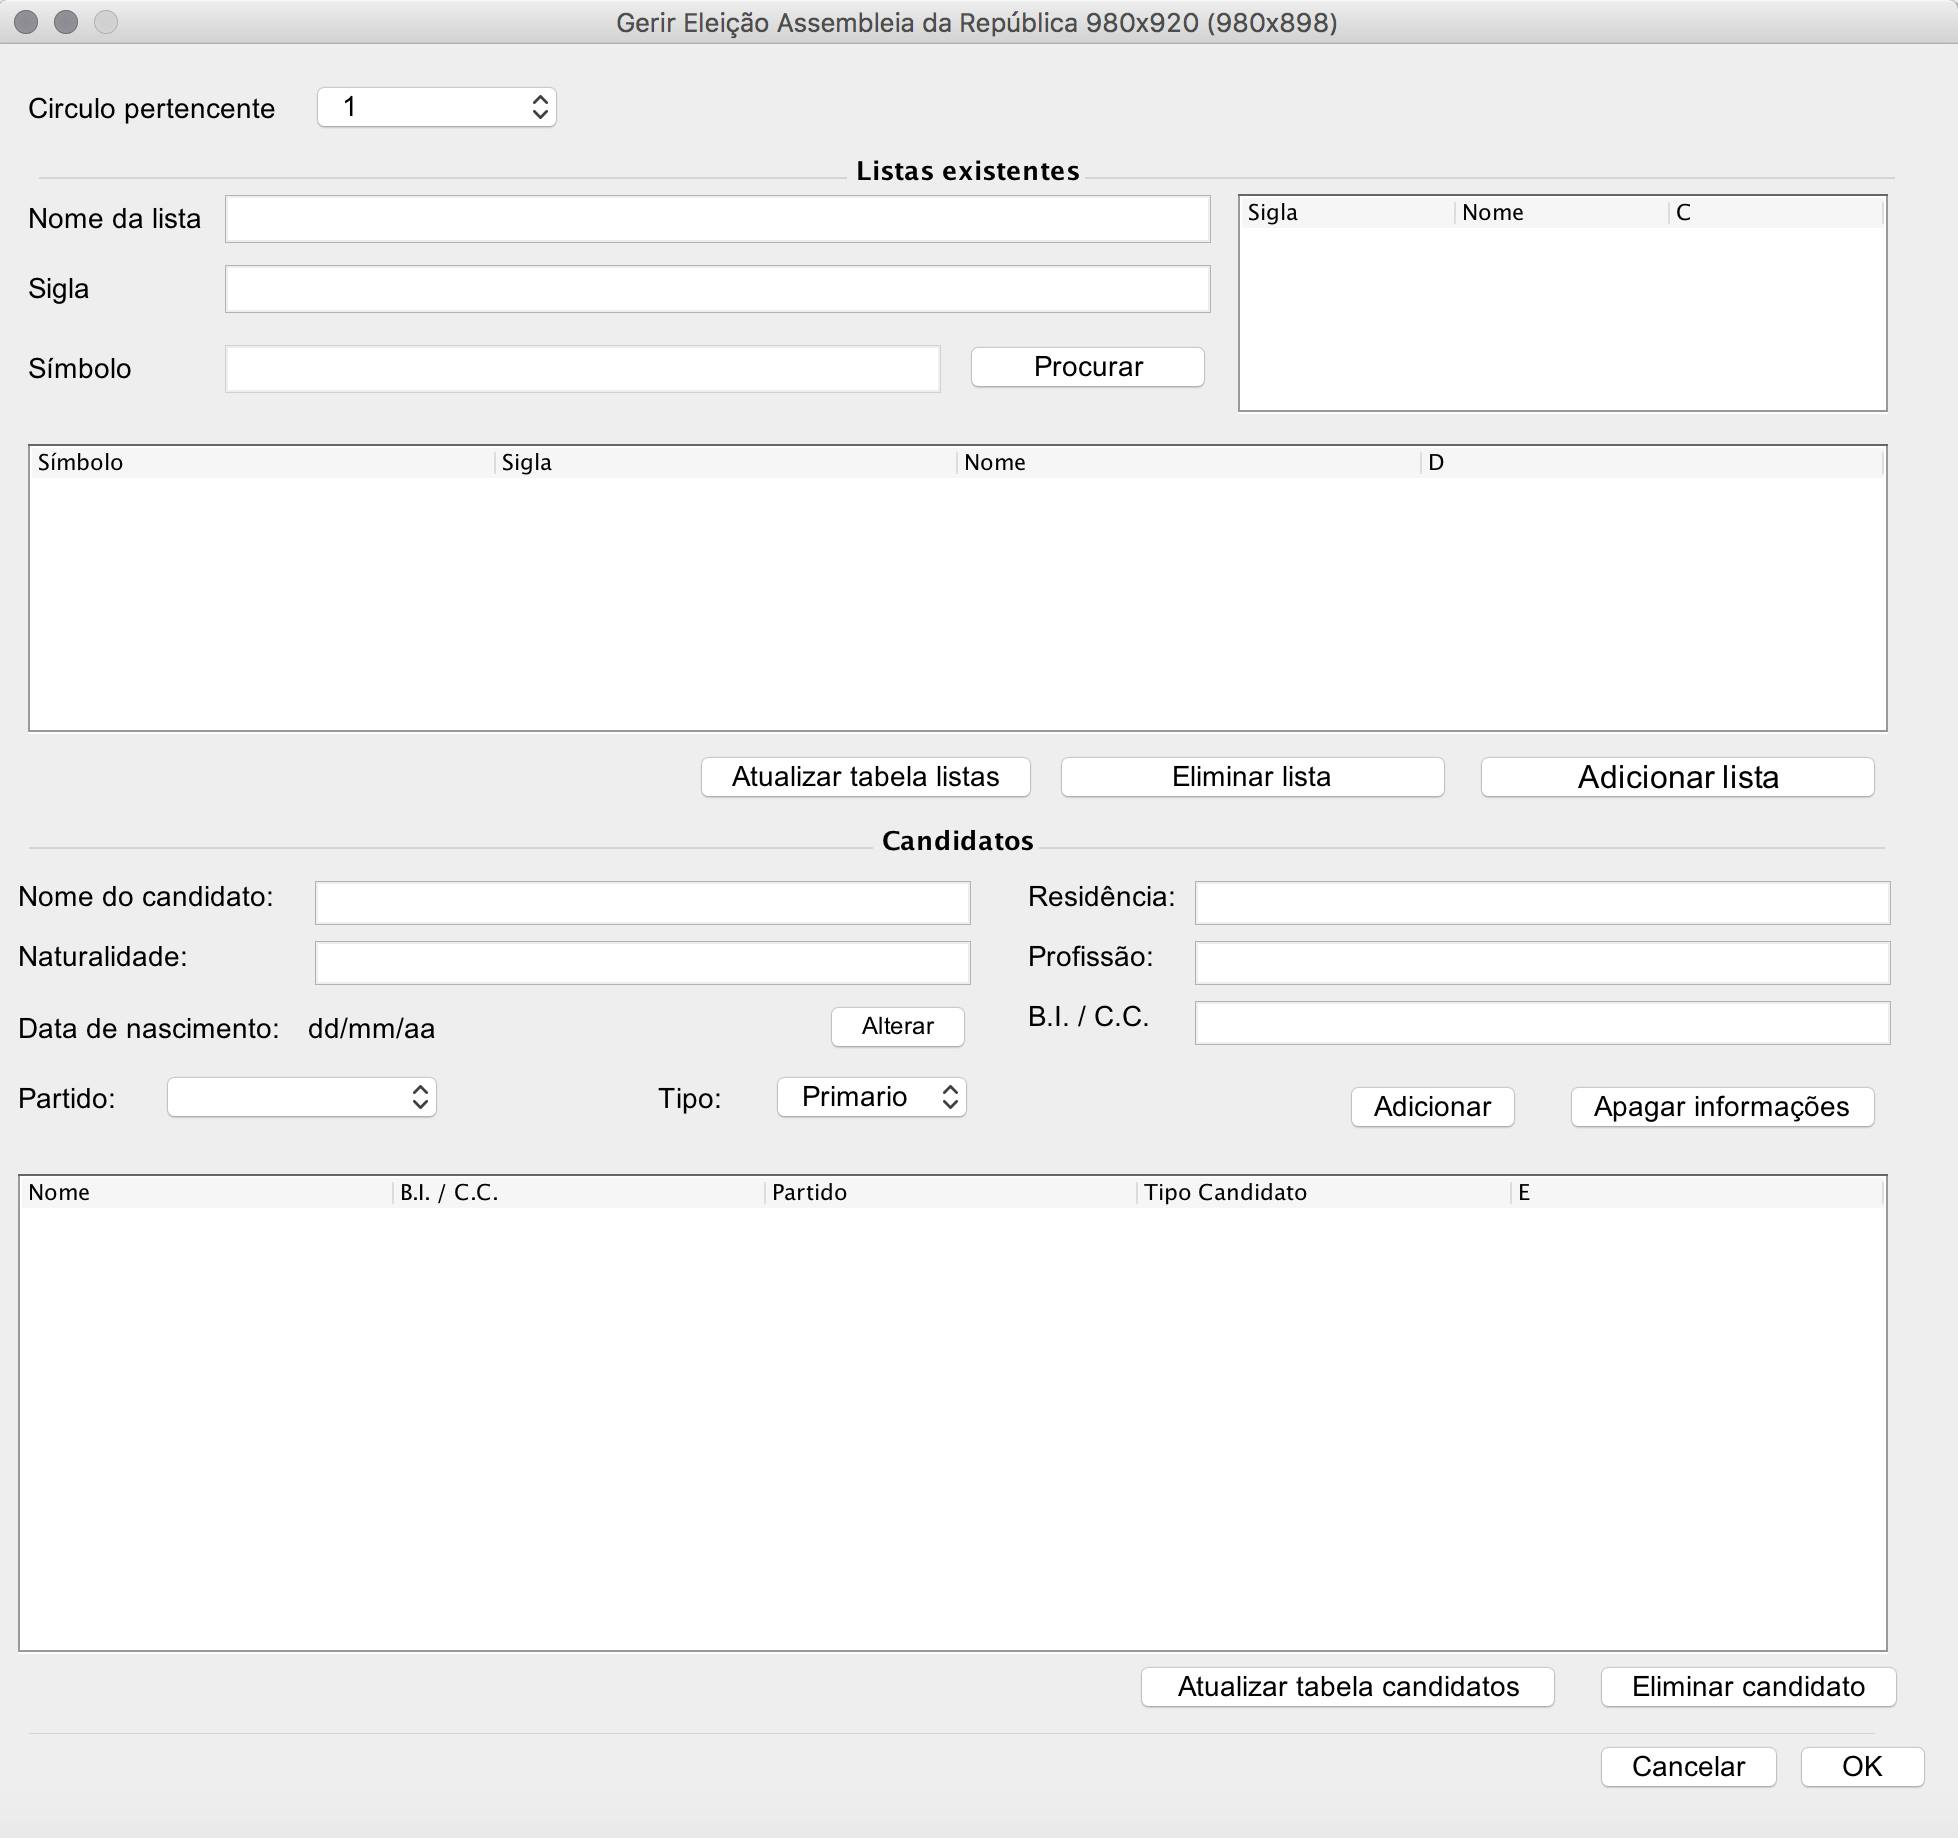
\includegraphics[width=0.5\textwidth]{media/img_interface/img11.jpg}
	 \caption{Gestão da Assembleia da República}
\end{center}
\end{figure}
\begin{figure}[H]
\begin{center}
	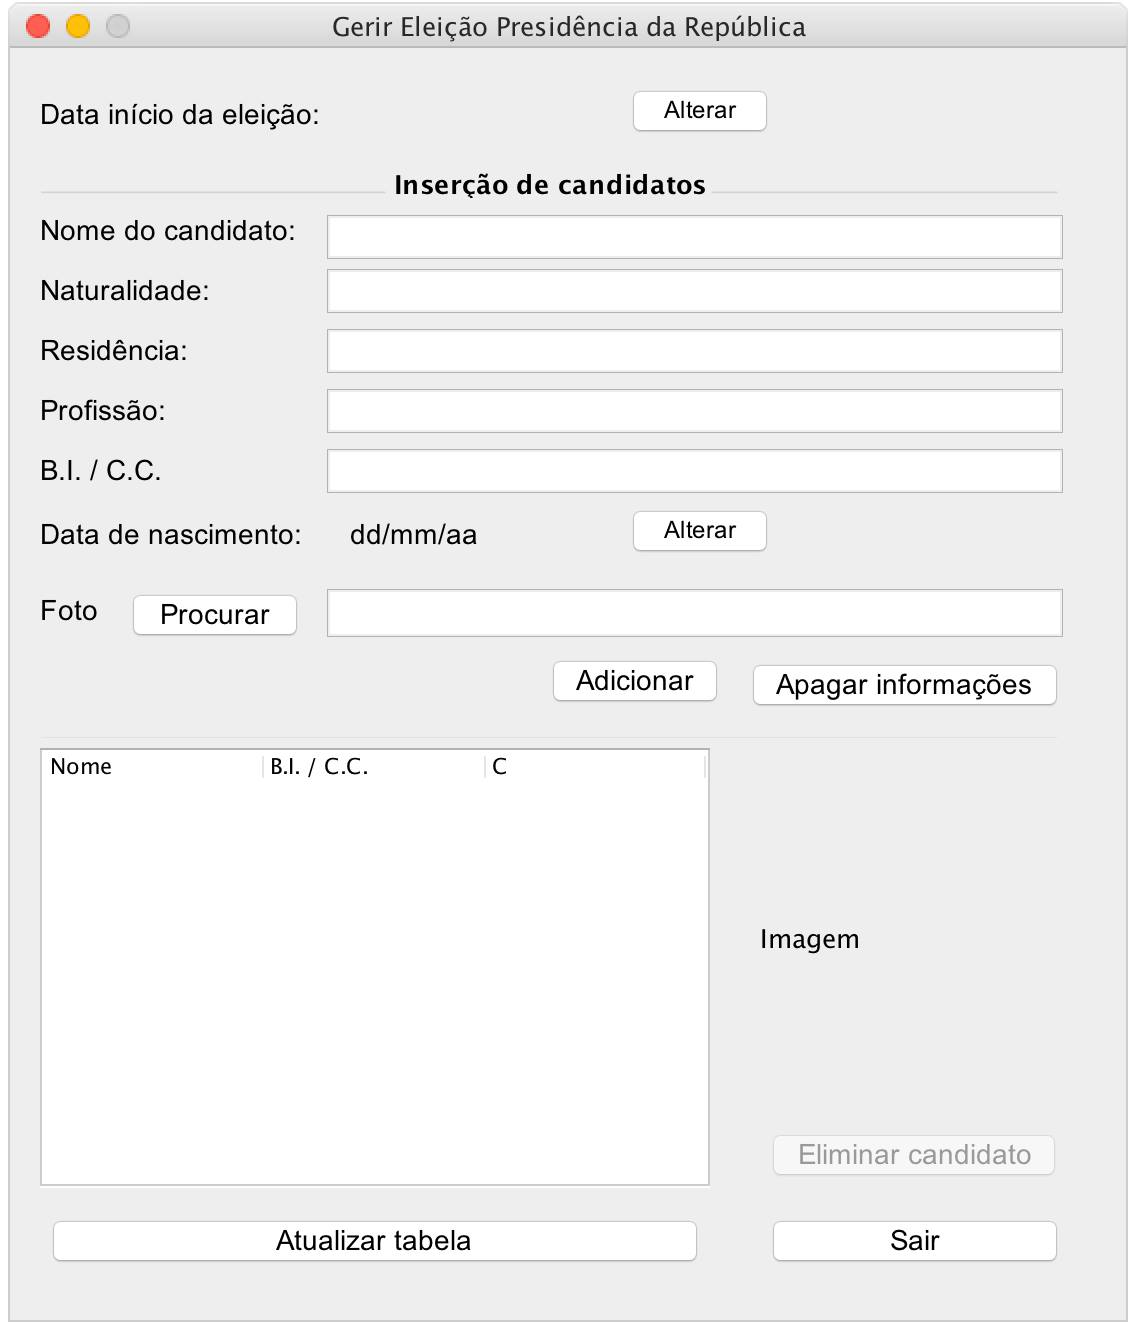
\includegraphics[width=0.5\textwidth]{media/img_interface/img7.jpg}
	 \caption{Gestão da Presidência da República}
\end{center}
\end{figure}
\newpage
\section{Decisões Estruturais}
Neta secção abordaremos algumas decisões que tomamos na execução do projeto que ainda não haviam sido referidas nas secções anteriores.
\\\indent Uma das preocupações que tivemos foi sempre que alguma alteração importante na aplicação ocorra, por exemplo um eleitor exerça o seu direito de voto, esta alteração no estado da aplicação seja refletida na persistência de dados. Isto ocorre para que não ser possível um eleitor votar mais que uma vez na mesma eleição. Esta decisão estrutural, numa futura iteração do modelo de desenvolvimento em espiral poderia ser otimizado para utilizar um sistema de \emph{cache}, que efetuaria a gestão inteligente das escritas em persistência. 
\\\indent Inexistência da classe Boletim na base de dados. De modo a utilizar menos recursos de bases de dados optamos por não introduzir na Base de Dados um mapeamento da entidade boletim que consideramos. Para solucionar esta decisão introduzimos em todos as classes \emph{Listáveis} pelo menos uma variável que representa o numero de ordem num boletim para que seja possível reconstruir um Boletim a qualquer momento de execução, incluindo na leitura dos dados das classes de persistência.
\\\indent Os DAO não implementam todos os métodos referidos na \emph{inteface} \emph{Map<K,V>}, com por exemplo o método 
\begin{verbatim}
public void putAll(Map<? extends K, ? extends V> m);
public Set<java.util.Map.Entry<Integer, Coligacao>> entrySet();
\end{verbatim}
uma vez que a sua implementação seria mais custosa para o grupo e tais métodos nunca seriam utilizados, o grupo achou que não havia necessidade de os definir. Contudo perto do fim e com alguma dificuldades na gestão das conceções à base de dados o grupo tomou em consideração que numa próxima iteração de desenvolvimento devirá ser implementado o método \emph{putALL()} para a \emph{class} \emph{EleitoresDAO} uma vez que os eleitores são as únicas entidade que são inseridas em massa na base de dados.  
\newpage
\section{Conclusão parte 2}
O nosso projeto está longe da perfeição devido à ambição da perfeição e ao elevado numero de funcionalidades que desejadas para a aplicação. 
\\\indent Caso existisse a possibilidade de começar o trabalho de novo, provavelmente simplificaríamos muita coisa como por exemplo a exibição dos resultados de uma Eleição de presidencia da republica por círculo, quando não era estritamente necessário.
\\\indent Relativamente à interface, uma vez que não temos elevados conhecimentos sobre o assunto, não se pode dizer que seja muito ``user-friendly'', que seria um aspeto passível de sofrer alterações.
\\\indent Inicialmente o grupo tinha como ideia de incluir na interface imagens dos candidatos e partidos ou coligações. No entanto, foram encontradas dificuldades devido ao facto de o o que ser guardado na base de dados ser a localização de uma imagem e não a imagem, o que leva a situações de erro sempre que a aplicação fosse executada em diferentes maquinas ou a imagem não estivesse disponível na mesma localização.
\\\indent Contudo, pensamos que este projeto da maneira que o abordamos, ficou um projeto mais extenso que o suposto, o que levou a que não ficasse desenvolvido a 100\% , as falhas que existem com mais algumas iterações do processo de desenvolvimento de software seguido poderiam ser colmatadas.
\\\indent De forma a terminar, todos os elementos do grupo estão de acordo em que os vários modelos utilizados são ferramentas poderosas no processo de modelação e desenvolvimento de sistemas. Tais processos permitem modelar o comportamento e estrutura do sistema, podendo ser interpretados por praticamente qualquer pessoa com os mínimos conhecimentos técnicos de engenharia de software. Este facto é muito importante para quem opta pelo modelo de implementação em espiral, pois facilita o processo de validação do desenvolvimento.


\newpage
\appendix
\section{Anexo}
\subsection{Modelo Lógico da Base de Dados} 
\begin{figure}[H]
	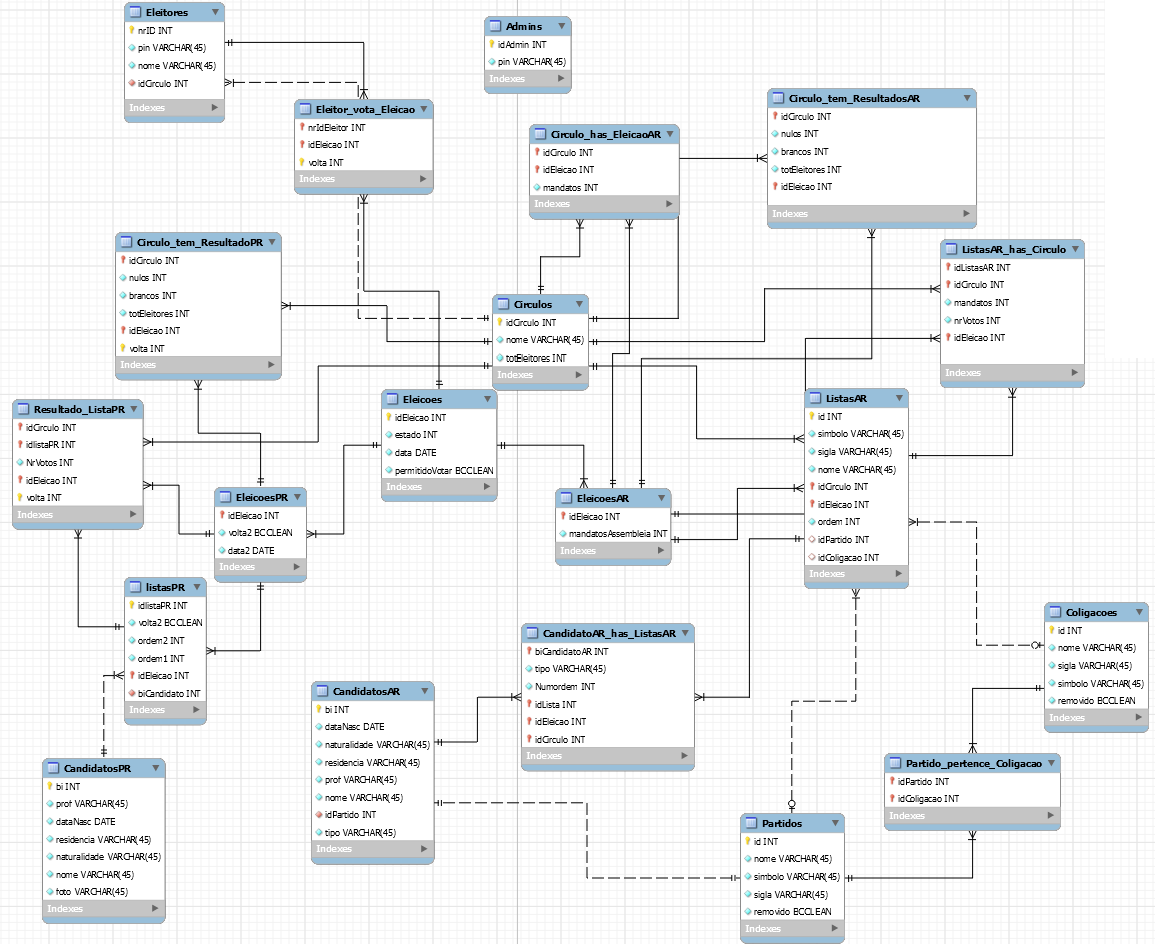
\includegraphics[width=1.2\textwidth]{media/modeloLogico/modelo_logico.png}
	 \caption{Modelo Lógico}
\end{figure}

\listoffigures
\begin{thebibliography}{1}
\bibitem{LeiPR}
LEI ELEITORAL do PRESIDENTE DA REPÚBLICA
\newblock{Decreto-Lei nº 319-A/76, de 3 de maio},
\newblock{acedida em 18/09/2015}.

\bibitem{LeiAR}
LEI ELEITORAL da ASSEMBLEIA DA REPÚBLICA
\newblock{Lei nº 14/79, de 16 de maio},
\newblock{acedida em 18/09/2015}.

\bibitem{slides}
José Creissac Campos, António Nestor Ribeiro, com contributos de F.M. Martins
\newblock{Desenvolvimento de Sistemas Software},
\newblock{MiEI – 3º ano / 1º semestre},
\newblock{2015/2016},

\end{thebibliography}

\end{document}
